%
% Copyright (c) 2001,2008 LAAS/CNRS
% All rights reserved.
%
% This document is a translation of the French documentation of GenoM,
% originally written by Sara Fleury and Matthieu Herrb.
%
% Redistribution  and  use in source   and binary forms,  with or without
% modification, are permitted provided that  the following conditions are
% met:
%
%   1. Redistributions  of  source code must  retain  the above copyright
%      notice, this list of conditions and the following disclaimer.
%   2. Redistributions in binary form must  reproduce the above copyright
%      notice,  this list of  conditions and  the following disclaimer in
%      the  documentation   and/or  other  materials   provided with  the
%      distribution.
%
% THIS SOFTWARE IS PROVIDED BY THE  AUTHOR AND CONTRIBUTORS ``AS IS'' AND
% ANY  EXPRESS OR IMPLIED WARRANTIES, INCLUDING,  BUT NOT LIMITED TO, THE
% IMPLIED WARRANTIES   OF MERCHANTABILITY AND  FITNESS  FOR  A PARTICULAR
% PURPOSE ARE DISCLAIMED.  IN NO  EVENT SHALL THE AUTHOR OR  CONTRIBUTORS
% BE LIABLE FOR ANY DIRECT, INDIRECT,  INCIDENTAL, SPECIAL, EXEMPLARY, OR
% CONSEQUENTIAL DAMAGES (INCLUDING,  BUT  NOT LIMITED TO, PROCUREMENT  OF
% SUBSTITUTE  GOODS OR SERVICES;  LOSS   OF  USE,  DATA, OR PROFITS;   OR
% BUSINESS  INTERRUPTION) HOWEVER CAUSED AND  ON ANY THEORY OF LIABILITY,
% WHETHER IN CONTRACT, STRICT LIABILITY, OR TORT (INCLUDING NEGLIGENCE OR
% OTHERWISE) ARISING IN ANY WAY OUT OF THE  USE OF THIS SOFTWARE, EVEN IF
% ADVISED OF THE POSSIBILITY OF SUCH DAMAGE.
%
%                                       Anthony Mallet on Thu Oct 18 2001
% $Id$
%

\documentclass[11pt]{book}

\usepackage{genom}		 % this document style
\usepackage{a4wide}
\usepackage{graphicx}
\usepackage{tabularx}
\usepackage{multirow}
\usepackage{varioref}

\makeatletter
\ifx\pdfoutput\@undefined\relax\else\ifnum\pdfoutput=1
   \usepackage[colorlinks=true,linkcolor=black,pagecolor=black]{hyperref}
\fi\fi
\makeatother
\usepackage[T1]{fontenc}
\usepackage[latin1]{inputenc}

\title{\fontsize{40}{40}\bf\GenoM\\\vskip1cm\Huge User's Guide}
\author{Sara Fleury, Matthieu Herrb, Anthony Mallet \\
LAAS-CNRS\\
7, Av. du Colonel Roche\\
31077 Toulouse Cedex 4 - France\\
{sara,matthieu,mallet}@laas.fr}

\date{August 2007}

\begin{document}

% -----------------------------------------------------------------------

\maketitle\thispagestyle{empty}

\tableofcontents

% -----------------------------------------------------------------------

\chapter*{\GenoM? What for?
\addcontentsline{toc}{chapter}{\protect\numberline{}GenoM? What for?}}
\label{cha|intro}
\markboth{\MakeUppercase{GenoM? What for?}}{}
%
% Copyright (c) 2001 LAAS/CNRS                        --  Thu Oct 18 2001
% All rights reserved.                                     Anthony Mallet
%
% This document is a translation of the French documentation of GenoM,
% originally written by Sara Fleury and Matthieu Herrb.
%
% Redistribution  and  use in source   and binary forms,  with or without
% modification, are permitted provided that  the following conditions are
% met:
%
%   1. Redistributions  of  source code must  retain  the above copyright
%      notice, this list of conditions and the following disclaimer.
%   2. Redistributions in binary form must  reproduce the above copyright
%      notice,  this list of  conditions and  the following disclaimer in
%      the  documentation   and/or  other  materials   provided with  the
%      distribution.
%
% THIS SOFTWARE IS PROVIDED BY THE  AUTHOR AND CONTRIBUTORS ``AS IS'' AND
% ANY  EXPRESS OR IMPLIED WARRANTIES, INCLUDING,  BUT NOT LIMITED TO, THE
% IMPLIED WARRANTIES   OF MERCHANTABILITY AND  FITNESS  FOR  A PARTICULAR
% PURPOSE ARE DISCLAIMED.  IN NO  EVENT SHALL THE AUTHOR OR  CONTRIBUTORS
% BE LIABLE FOR ANY DIRECT, INDIRECT,  INCIDENTAL, SPECIAL, EXEMPLARY, OR
% CONSEQUENTIAL DAMAGES (INCLUDING,  BUT  NOT LIMITED TO, PROCUREMENT  OF
% SUBSTITUTE  GOODS OR SERVICES;  LOSS   OF  USE,  DATA, OR PROFITS;   OR
% BUSINESS  INTERRUPTION) HOWEVER CAUSED AND  ON ANY THEORY OF LIABILITY,
% WHETHER IN CONTRACT, STRICT LIABILITY, OR TORT (INCLUDING NEGLIGENCE OR
% OTHERWISE) ARISING IN ANY WAY OUT OF THE  USE OF THIS SOFTWARE, EVEN IF
% ADVISED OF THE POSSIBILITY OF SUCH DAMAGE.
%
% $Id$
%

\GenoM\ (\textbf{Gen}erator \textbf{o}f \textbf{M}odules) is a development
framework that allows  the definition and the  production of modules that
encapsulate algorithms.  A module is  a standardized software entity that
is able to offer services which are provided by your algorithms.  Modules
can start or stop the execution of these services,  pass arguments to the
algorithms and export the data produced.

Now  you  might ask  yourself:  ``why should  I bother  integrating  into
modules my   own algorithms that   \emph{do} work  very  well?''. That's a
pretty good  question and this introduction  will try to advocate on that
point and give you some answers.

\bigbreak

Your  algorithms aim to  being embedded into  a  \emph{target} machine ---
let's say: a robot.  You might not embrace the way  this machine works in
its whole and, most important, your  algorithms will be integrated into a
more general software system that includes  other algorithms developed by
other persons.  This set of  algorithms  share several common properties:
they must be configured (don't you have a bunch of parameters you want to
adjust?), they must be started, interrupted, started again or stopped and
we might expect them to exchange data and communicate  with other part of
the system.

Consider the example of a mobile  robot: depending on the requirements of
its mission and the current context of execution, the robot might need to
acquire an image, localize itself,  build a local  map with some  sensors
and  move.  If the  environment  is rather free, the  robot  could plan a
trajectory, but  it could also  decide to move on the  basis of the local
data given by its  proximetric  sensors.  To be   able to schedule  these
rather complex (and uncertain!) actions, it  is \emph{necessary} to define
a protocol that can handle tasks at an abstract level. This protocol will
let the robot:

\begin{itemize}
\item start an action when it is needed;
\item stop an action in a clean manner;
\item pass a set of parameters and data to the action;
\item coordinate several actions;
\item get the results of these actions;
\item handle the failures of the actions (yes, actions can fail!) an keep
them from  taking the whole system with them when they spiral
down. Failures can be as general as:
   \begin{itemize}
   \item low batteries,
   \item incorrect algorithm parameters,
   \item not enough memory to handle that case,
   \item the target to localize does not appear in the images,
   \item the algorithm cannot handle that situation yet,
   \item \ldots
   \end{itemize}
\end{itemize}

Therefore,  the  general   concept  of  \emph{module}  and   \emph{standard
protocols}  have  been defined.   These  generic  modules can encapsulate
almost  every  kind of  algorithm:  periodic or aperiodic, synchronous or
asynchronous, interruptible or uninterruptible, and even yours!

Of course, you could yourself write a module on the basis of that generic
model. But that's a long and difficult story: you will  have to port your
software on the different systems you want it to run on, you will have to
write  test procedures to  check that  your  module behaves correctly  in
every situation, \ldots\ and \GenoM\ already does it for you!

\bigbreak

The generator  of modules comes  with  a description \emph{language},  and
standard templates.  The templates will let you describe your module, the
services  it  can offer, and  for   each  service the  list  of  expected
parameters,  the algorithms (yours!) that will  be  executed, the results
along with their description, the failure messages and a few other items.

With the template file and the code of your algorithms --- sorry, you still
must write it yourself --- \GenoM\ produces:

\begin{itemize}
   \item \emph{a complete module} that can run on several flavor of Unix
or VxWorks, 
   \item \emph{interface libraries} that will let you use the services of
the module and get their results back,
   \item \emph{an interactive test program} that let you send several
requests to the module and trigger the execution of the corresponding
services.
\end{itemize}

\bigbreak

Now that you  have an idea  of what \GenoM\ can  be used for, this manual
will explain you \emph{how} to actually do it. You will learn

\begin{center}\begin{cartouche}\parbox{0.9\hsize}{
\parskip10pt
    1. \textbf{How to produce and use a first test module}, with a concrete
example.

    2. \textbf{How the generic modules work}, and \textbf{how they are
structured}. In particular, some useful vocabulary is explained.

    3. \textbf{How to describe your own modules}. The complete
specification language will be explained.

    4. \textbf{How to generate your modules}.

    5. \textbf{How to integrate your algorithms into the modules}.

    6. \textbf{How to use modules} (from an interactive program, from
another module, \ldots).
}\end{cartouche}\end{center}



\chapter{Installation and configuration}
\label{cha|configuration}
%
% Copyright (c) 2001-2005 LAAS/CNRS                   --  Sat Nov 19 2005
% All rights reserved.                                     Sara Fleury
%
% This document is a translation of the French documentation of GenoM,
% originally written by Sara Fleury and Matthieu Herrb.
%
% Redistribution  and  use in source   and binary forms,  with or without
% modification, are permitted provided that  the following conditions are
% met:
%
%   1. Redistributions  of  source code must  retain  the above copyright
%      notice, this list of conditions and the following disclaimer.
%   2. Redistributions in binary form must  reproduce the above copyright
%      notice,  this list of  conditions and  the following disclaimer in
%      the  documentation   and/or  other  materials   provided with  the
%      distribution.
%
% THIS SOFTWARE IS PROVIDED BY THE  AUTHOR AND CONTRIBUTORS ``AS IS'' AND
% ANY  EXPRESS OR IMPLIED WARRANTIES, INCLUDING,  BUT NOT LIMITED TO, THE
% IMPLIED WARRANTIES   OF MERCHANTABILITY AND  FITNESS  FOR  A PARTICULAR
% PURPOSE ARE DISCLAIMED.  IN NO  EVENT SHALL THE AUTHOR OR  CONTRIBUTORS
% BE LIABLE FOR ANY DIRECT, INDIRECT,  INCIDENTAL, SPECIAL, EXEMPLARY, OR
% CONSEQUENTIAL DAMAGES (INCLUDING,  BUT  NOT LIMITED TO, PROCUREMENT  OF
% SUBSTITUTE  GOODS OR SERVICES;  LOSS   OF  USE,  DATA, OR PROFITS;   OR
% BUSINESS  INTERRUPTION) HOWEVER CAUSED AND  ON ANY THEORY OF LIABILITY,
% WHETHER IN CONTRACT, STRICT LIABILITY, OR TORT (INCLUDING NEGLIGENCE OR
% OTHERWISE) ARISING IN ANY WAY OUT OF THE  USE OF THIS SOFTWARE, EVEN IF
% ADVISED OF THE POSSIBILITY OF SUCH DAMAGE.
%

% -----------------------------------------------------------------------

\section{Quick start using robotpkg}

The robotpkg\footnote{\url{http://robotpkg.openrobots.org/}} tool is
the quickest way to install GenoM and its dependencies. 

\subsection{Setting up robotpkg in five minutes}


After downloading the sources, you need to choose where the packages
will be installed and bootstrap your installation. For that, you need
the GNU make software (version 3.81 or later required), as well as a
working C compiler chain.

By default, robotpkg uses the \texttt{/opt/openrobots} installation prefix. If
this location is convenient for you, installing the bootstrap kit
should be as simple as:

\begin{cartouche}
\begin{verbatim}
% cd robotpkg/bootstrap
% ./bootstrap
\end{verbatim}
\end{cartouche}

Notes:
\begin{itemize}
\item The bootstrap script will try to create the initial
  /opt/openrobots directory using your user id. You are usually not
  allowed to do so, so you should create the /opt/openrobots manually
  before calling bootstrap (using sudo or a similar command). You can
  also install to a different location as explained below. 

\item If you need to install to a different prefix, pass the --prefix
  option to bootstrap. For instance, installing the packages in your
  home directory can be configured like this: 

\begin{cartouche}
\begin{verbatim}
      % ./bootstrap --prefix=${HOME}/openrobots
\end{verbatim}
\end{cartouche}
\end{itemize}

Make sure to read carefuly the instructions printed at the end of the bootstrap for configuring your shell environment.

\subsection{The five minutes guide to installing Genom}

Once bootstraping is done, installing a package can be done by
changing to the directory (within the robotpkg hierarchy) of the
package to be installed and doing make update. For GenoM, this means:

\begin{cartouche}
\begin{verbatim}
% cd robotpkg/architecture/genom
% make update
\end{verbatim}
\end{cartouche}


Notes:
\begin{itemize}
\item The make program must be GNUmake utility, a.k.a gmake. Version
  >= 3.81 is required.  
\end{itemize}

A more extensive and largely incomplete (!) documentation is also
available
online\footnote{\url{http://robotpkg.openrobots.org/}},
or in the \texttt{doc/robotpkg} directory of robotpkg. 

If you successfully installed GenoM with robotpkg, you can skip to the
next chapter. Otherwise read more detailled instructions below.

\section{Requirements}
\label{sec|configuration|requirements}

\subsection{Operating systems}

GenoM is known to work on most current Unix-like operating systems:
Linux (many distributions including Debian, Fedora, Gentoo and Ubuntu
have been tested), NetBSD, Mac OS X, Solaris.

GenoM does not work on Microsoft Windows operating system, nor on
mobile phones / tablets operating systems like Apple's iOS or Google's
Android. 

\subsection{External tools}

GenoM needs the following tools.
They are generally available on most systems. If not, download
them from their web sites. 

\begin{itemize}
\item \texttt{autoconf} version 2.59 or later
\item \texttt{automake} version 1.8 or later
\item \texttt{GNU make} version 3.79 or later  (\texttt{<http://www.gnu.org/software/make/make.html>})
\item \texttt{pkgconfig} version 0.15 or later (usually part of Gnome development packages).
\item \texttt{groff} 1.10 or later (usually part of system packages).
\item \texttt{Tcl/Tk} 8.0 or later development files (for eltclsh) (\texttt{<http://tcl.tk/>})
\end{itemize}

To edit GenoM modules it is also recommended to use \texttt{xemacs} to take
advantage of \texttt{genom-mode}.

\section{What to download ?}
\label{sec|configuration|download}

\subsection{OpenRobots tools and libraries}

GenoM is part of a suite of open-sources tools. 

In order to install and use GenoM you will have to download and install
the following libraries and tools from  
\texttt{https://git.openrobots.org/} :

\begin{itemize}
\item \texttt{mkdep}: LAAS tool to determine dependencies
\item \texttt{pocolibs}: system communication and real-time primitives
\item \texttt{libedit} (editline): generic line editing and history
functions (for eltclsh)
\item \texttt{eltclsh}: interactive TCL shell linked with editline (optional but very practical)
\item \texttt{GenoM}: the generator of modules
\end{itemize}

Later on you can also be interested in the following opensource softwares
that are part of the OpenRobots suite and work nicely with GenoM:

\begin{itemize}
\item \texttt{GDHE}: a tool to design 3D interface
\item \texttt{OpenPRS}: a tool to design complexe supervisors
\end{itemize}

\subsubsection{mkdep}

\texttt{Mkdep} is a tool to manage dependencies for make(1) automatically on
Unix-like systems.  The original feature of this version is to be able to
handle incremental updates of the dependencies.

It is recommended to install it.

\subsubsection{pocolibs}

\texttt{Pocolib} is a system communication and real-time primitive layers used by
GenoM modules. 

These libraries run on systems with POSIX.1 threads and basic real-time
extensions. It has been tested successfully on Solaris (7 and above),
Linux (with glibc2), and NetBSD (2.0 and later). 

There is also some code to support RTAI and LXRT 3.0, but it is currently
untested and unsupported (this may change again in the future) 

\subsubsection{tclserv}

Starting with \GenoM{} version 2.7, \texttt{tclserv} is provided as an
external package. It will need to be installed separately to be able
to use it as described in section~\ref{sec|tcl}.

\subsubsection{libedit / editline}

The \texttt{editline} library provides generic line editing and history
functions, similar to those found in tcsh(1). This package contains a
Makefile for compiling the current version of NetBSD's library which
provides the same consistent installation and compilation environments as
for the other tools found in this repository. 

Editline is used by eltclsh.

\subsubsection{eltclsh}


% -----------------------------------------------------------------------
\section{Configuration}
\label{sec|configuration|configuration}


You will need to specify a root path (for instance the environment
variable \texttt{OPENROBOTS}) where the binaries, the libraries, the
include files, and so on will be installed. Typically you can set this
environment variable to \texttt{/usr/local/openrobots}.

Then modify (or set if not previously defined) the following 
environment variables :

\texttt{PATH} :  add \texttt{\$OPENROBOTS/bin}

\texttt{PKG\_CONFIG\_PATH} :  add  \texttt{\$OPENROBOTS/lib/pkgconfig}

\texttt{LD\_LIBRARY\_PATH} :  add  \texttt{\$OPENROBOTS/lib:\$OPENROBOTS/lib/openprs}



% -----------------------------------------------------------------------
\section{Installation}
\label{sec|configuration|installation}

Most of the time, it is a simple sequence of untar, autogen, configure,
build, and install. Configure options may vary, and some packages don't
require the autogen step. It is recommended that you build in a separate
directory. 

The \texttt{--prefix} option (default: /usr/local) defines the base directory
of the installation. We recommend a dedicated path (eg,
OPENROBOTS=/usr/local/openrobots).

If you want to install binaries for different type of machine
on the same files tree you can also use \texttt{--exec-prefix}
option. It allows to specify where to install the binaries like for
instance: \texttt{--exec-prefix=\$OPENROBOTS/\$MACHTYPE-\$OSTYPE} (eg,
\texttt{--exec-prefix=\$OPENROBOTS/i386-linux}, for a PC running linux).
In such a case, be careful to adapt the environment variables 
\texttt{PATH, LD\_LIBRARY\_PATH and PKG\_CONFIG\_PATH} defined above to this
\texttt{\$exec\_prefix} path.
%$
However, the default value (equal to \texttt{--prefix}) is usualy great. 


Here is an
example with \texttt{pocolibs}. 

\begin{cartouche}
\begin{verbatim}
tar xfvz pocolibs-XYZ.tar.gz
cd pocolibs-XYZ
[./autogen.sh]
mkdir build
cd build
../configure --prefix=\$OPENROBOTS  %$
make
make install
\end{verbatim}
\end{cartouche}

The command \texttt{./autogen.sh} is not always necessary. If there is
already a \texttt{configure} script  you can try it directly.

On some systems, \texttt{--with-tcl=DIR} and \texttt{--with-tk=DIR} will be
required to specify where to find \texttt{tclConfig.sh} (resp. \texttt{tkConfig.h}). 

The \texttt{configure} command has many options. You can see them with the
option \texttt{--help}. 




\chapter{A first example}
\label{cha|session}
%
% Copyright (c) 2001 LAAS/CNRS                        --  Thu Oct 18 2001
% All rights reserved.                                     Anthony Mallet
%
% This document is a translation of the French documentation of GenoM,
% originally written by Sara Fleury and Matthieu Herrb.
%
% Redistribution  and  use in source   and binary forms,  with or without
% modification, are permitted provided that  the following conditions are
% met:
%
%   1. Redistributions  of  source code must  retain  the above copyright
%      notice, this list of conditions and the following disclaimer.
%   2. Redistributions in binary form must  reproduce the above copyright
%      notice,  this list of  conditions and  the following disclaimer in
%      the  documentation   and/or  other  materials   provided with  the
%      distribution.
%
% THIS SOFTWARE IS PROVIDED BY THE  AUTHOR AND CONTRIBUTORS ``AS IS'' AND
% ANY  EXPRESS OR IMPLIED WARRANTIES, INCLUDING,  BUT NOT LIMITED TO, THE
% IMPLIED WARRANTIES   OF MERCHANTABILITY AND  FITNESS  FOR  A PARTICULAR
% PURPOSE ARE DISCLAIMED.  IN NO  EVENT SHALL THE AUTHOR OR  CONTRIBUTORS
% BE LIABLE FOR ANY DIRECT, INDIRECT,  INCIDENTAL, SPECIAL, EXEMPLARY, OR
% CONSEQUENTIAL DAMAGES (INCLUDING,  BUT  NOT LIMITED TO, PROCUREMENT  OF
% SUBSTITUTE  GOODS OR SERVICES;  LOSS   OF  USE,  DATA, OR PROFITS;   OR
% BUSINESS  INTERRUPTION) HOWEVER CAUSED AND  ON ANY THEORY OF LIABILITY,
% WHETHER IN CONTRACT, STRICT LIABILITY, OR TORT (INCLUDING NEGLIGENCE OR
% OTHERWISE) ARISING IN ANY WAY OUT OF THE  USE OF THIS SOFTWARE, EVEN IF
% ADVISED OF THE POSSIBILITY OF SUCH DAMAGE.
%
% $Id$
%

A module is described with a particular syntax  in a file whose name ends
in ``dot   gen'' ({\tt .gen}).  In this   chapter, we will  write  a test
module which we will call ``demo''.  Thus the file describing this module
will be  called  {\tt demo.gen}.  The next  sections  explain  how such a
module is generated and used.

% -----------------------------------------------------------------------
\section{Principle of the module generation}
\label{sec|session|principle}

One can distinguish two main parts in a module:

\begin{itemize}
   \item A {\em server}, which encapsulate algorithms and is generated
automatically by \GenoM\ from the description file,
   \item The set of {\em algorithms} that you have developed, and that
will be included into the module.
\end{itemize}

To combine these two parts and form  a complete module, the definition of
functions that  will interface the server and  the algorithms together is
required (at the moment  only {\tt  C}  functions are  supported).  These
functions are  called ``codels'' (which  stands for {\em code elements}),
and they represent the {\em smallest} grain size  the server will be able
to manipulate.

The first  time \GenoM\  is called,  it generates empty  codels. They are
fully  functional, but do  nothing. It's up to  you to fill  them in with
your own code.

\bigbreak

\begin{figure}[htbp]
\centering
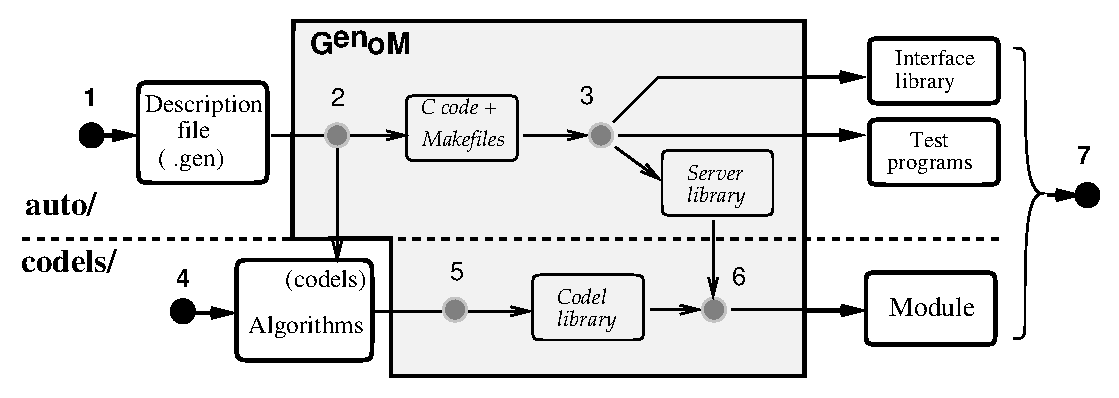
\includegraphics[width=0.8\hsize]{fig/cycle-en}
\caption{Development cycle and separation between sever and codels.}
\label{fig|session|cycle}
\end{figure}

To help   you distinguish  between   the  server   and the   codels,  the
corresponding files are placed in two separate directories. The first one
is called {\tt server/} and contains all  the code generated by \GenoM. The
second directory is called {\tt   codels/} and  contains the codels   ---
initially a template generated by \GenoM\ but never touched again once
you have filled them in.

\bigbreak

The figure~\ref{fig|session|cycle} shows a synthetic view of the
separation between {\tt server/} and {\tt codels/} and also represent a
typical development cycle~:

\begin{description}
   \item{\bf 1. module description:} edition of the {\tt .gen} file,
   \item{2. and 3. server generation and compilation},
   \item{\bf 4. write the codels that will invoke your algorithms},
   \item{5. and 6. compile the codels and link with the server},
   \item{\bf 7. test and use the module}.
\end{description}

Only the points {\bf 1}, {\bf 4} and {\bf  7} are in your charge. \GenoM\
writes for you   the {\tt Makefile}s  and  handle the compilation of  the
various files.

Once you have  compiled a module,  you  can incrementally modify, add  or
remove services (back to  the first point) and  codels (back to the point
number 4).

% -----------------------------------------------------------------------
\section{An example}
\label{sec|session|example}

This section will  illustrate a concrete use  of \GenoM\ with  a ``demo''
module. This module  will  control a  mobile that  can translate  on  a 2
meters long rail. Some of the services the ``demo'' module offers are:

\begin{itemize}
   \item select the speed (between two symbolic values {\tt DEMO\_SLOW}
and {\tt DEMO\_FAST}),
   \item move the mobile for a given distance,
   \item read the current speed or position at any moment,
   \item suspend the motion,
   \item monitor particular positions and inform when the mobile goes
through these positions.
\end{itemize}

To implement this, we first create a directory named {\tt demo/}. In that
directory we will write the description file {\tt demo.gen}, which could
look like this (see next page):
\vfill\eject

\vbox to\textheight{\vfill
\begin{center}
\begin{cartouche}\small
\begin{verbatim}
/* -------------------------- MODULE DECLARATION --------------------------- */

module demo {
   number:            9000;            /* module id: unique number */
   internal_data:     DEMO_STR;        /* C typedef (defined below) */
};


/* ------------- DEFINITION OF THE MODULE's INTERNAL DATABASE -------------- */

/* External definitions involved in the database definition */
#include "demoStruct.h"

/* The internal database */
typedef struct DEMO_STR {
   DEMO_STATE_STR   state;           /* Current state of the mobile */
                                     /* (position and speed) */
   DEMO_SPEED       speedRef;        /* Speed reference */
   double           distRef;         /* Distance reference */
   double           monitor;         /* Positions monitors */
}DEMO_STR;
 

/* ------------------ SERVICES DEFINITION: The REQUESTS -------------------- */

/* Control request: modify the default speed */
request SetSpeed {
   type:                control;              /* request's type  */
   input:               speed::speedRef;      /* input: speed chosen */
   c_control_func:      demoControlSpeed;     /* codel for validity checks */
   fail_msg:            INVALID_SPEED;        /* possible error messages */
};

/* Control request: return the default speed */
request GetSpeed {
   type:                control;              /* request's type */
   output:              speed::speedRef;      /* output: the speed */
};

/* Control request:  interrupt the mobile */
request Stop {
   type:                control;              /* request's type */
   incompatible_with:   MoveDistance;         /* request to interrupt */
};
\end{verbatim}
\end{cartouche}
\end{center}
\vfill
\hfill continued on next page...
}
\eject

\vbox to\textheight{
... continuation of previous page
\vfill
\begin{center}
\begin{cartouche}\small
\begin{verbatim}
/* Execution request: translate of a given distance */
request MoveDistance {
   type:                exec;                 /* request's type */
   input:               distance::distRef;    /* input: distance */
   c_control_func:      demoControlDistance;  /* codel for validity checks */
   fail_msg:            TOO_FAR_AWAY;         /* possible error messages */
   c_exec_func_start:   demoStartEngin;       /* initialization codel */
   c_exec_func:         demoGotoPosition;     /* main codel */
   c_exec_func_end:     demoStopEngin;        /* termination codel */
   c_exec_func_inter:   demoStopEngin;        /* interruption codel */
   incompatible_with:   MoveDistance;         /* incompatible requests */
   exec_task:           MotionTask;           /* task (thread) executing
                                               * the codel */
};

/* Execution request: monitor a particular mobile's position */
request Monitor {
   type:                exec;                 /* request's type */
   input:               position::monitor;    /* inputs: position */
   output:              position::state.position; /* outputs: actual pos. */
   c_exec_func:         demoMonitor;          /* main codel */
   fail_msg:            TOO_FAR_AWAY;         /* possible error messages */
   incompatible_with:   none;                 /* no incompatible requests */
   exec_task:           MotionTask;           /* task (thread) */
};


/* ------------------------ POSTERS DECLARATION  --------------------------- */

/* Poster that exports the current state of the mobile */
poster Mobile {
   update:               auto;
   data:                 state::state, ref::distRef;
   exec_task:            MotionTask;
};

 
/* --------------------- EXECUTION TASKS DECLARATION ----------------------- */

/* Only one task (or thread) */
exec_task MotionTask {
   period:               20;
   delay:                0;
   priority:             100;
   stack_size:           2000;
   c_init_func:          demoInit;
};
\end{verbatim}
\end{cartouche}
\end{center}
\vfill
}
\eject

The file {\tt demo.gen} is made up of five parts, each of them being
identified with a keyword (these keywords are explained in detail in
chapter \ref{cha|edit}):

\begin{center}\begin{tabular}{llll}
1.& {\tt module} & module declaration \\
\noalign{\vskip10pt}

2.& \parbox[t]{4cm}{
\hbox{\tt \#include} and
\hbox{\tt typedef struct}} & \parbox[t]{9cm}{{\tt C} include
statement for the definition of structures and declaration of the
internal database} \\
\noalign{\vskip10pt}

3.& {\tt request} & \parbox[t]{9cm}{requests definition: the five
services offered by the module} \\
\noalign{\vskip10pt}

4.&  {\tt   poster} & \parbox[t]{9cm}{posters  definition:   posters  are
exported  data structures  that let information  on the  mobile  state be
available for other modules} \\
\noalign{\vskip10pt}

5.& {\tt exec\_task} & \parbox[t]{9cm}{execution task declaration (a
thread for Unix) that take care of codel execution}\\
\end{tabular}\end{center}

\bigbreak

The {\tt \#include demoStruct.h} statement (the  second part above) works
as in {\tt C} and  includes the corresponding {\tt  C} header file.  This
file contains   all the necessary   {\tt  typedef} declarations  for  the
definition of the  internal database. These structures  are  then used by
the {\tt request} and the {\tt poster} declarations.

In this example,  the file {\tt  demoStruct.h} contains the definition of
{\tt  DEMO\_STATE\_STR} and  {\tt DEMO\_SPEED}. This   file is preferably
located in the same directory as {\tt demo.gen},  since it contributes to
the definition of the module interface.

\bigbreak

\begin{center}
\begin{cartouche}\small
\begin{verbatim}
#ifndef DEMO_STRUCT_H
#define DEMO_STRUCT_H

/* Current state of the mobile */
typedef struct DEMO_STATE_STR {
   double position;              /* current position */
   double speed;                 /* current speed */
}DEMO_STATE_STR;

/* Admissible speeds */
typedef enum DEMO_SPEED{
  DEMO_SLOW,                     /* low speed */
  DEMO_FAST                      /* high speed */
} DEMO_SPEED;

#endif /* DEMO_STRUCT_H */
\end{verbatim}
\end{cartouche}
\end{center}


% -----------------------------------------------------------------------
\section{Module generation}
\label{sec|session|generate}

The  generation step is done  through the {\tt genom} command invocation.
When a module is to be generated for the  first time, {\tt genom} must be
invoked  with the {\tt  -i} option, which installs  the initial files (in
particular, it installs the codels templates).  Here is a sample run, for
the {\tt demo} example:

\begin{center}
\begin{cartouche}\small
\begin{verbatim}
blues% genom  -t demo
genom demo.gen: info: array MonitorInput added in SDI for request Monitor
genom demo.gen: info: array MonitorOutput added in SDI for request Monitor
perl -w ./demo.pl

Updating top directory
  creating acinclude.user.m4
  creating local.mk.in
  creating configure.ac.user
  creating autogen
  creating Makefile.in

Updating codels
  demoMotionTaskCodels.c changed, skipping
  demoCntrlTaskCodels.c changed, skipping
  Makefile.in changed, skipping

Updating autoconf
  creating genom.mk
  creating install-sh
  creating mkinstalldirs
  creating config.sub
  creating config.guess
  creating ltmain.sh
  creating robots.m4
  creating libtool.m4
  creating config.posix.mk
  creating config.rtai.mk

Updating server
  creating Makefile.in
  creating demoType.h
  creating demoError.h
  creating demoError.c
  creating demoMsgLib.c
  creating demoConnectLib.c
  creating demoMsgLib.h
  creating demoMsgLibProto.h
...
Creating build environment ...
  * Running aclocal
  * Running autoconf


If you already have a build of this module, do not forget to
reconfigure (for instance by running ./config.status --recheck)

Done.

\end{verbatim}
\end{cartouche}
\end{center}

\bigbreak

Some comments on this run:

\begin{enumerate}
   \item  The {\tt   .gen}  extension   needs   not  to be    explicitely
   given. \GenoM\ appends it automatically.


   \item \GenoM\ creates two directories and a great number of files. You
   do not need to know them all, and they will be described later in this
   document (they are also described in the appendix \ref{anx|files}).
\end{enumerate}

{\bf From now on, the module is ready to  be compiled and run}, but let's
look at the result of the execution of {\tt genom}:

\begin{center}
\begin{cartouche}\small
\begin{verbatim}
blues% ls -F
CVS/               autoconf/  configure*         demoConst.h   server/
Makefile.in        autogen*   configure.ac.user  demoStruct.h  xaff/
acinclude.user.m4  codels/    demo.gen           local.mk.in
\end{verbatim}
\end{cartouche}
\end{center}

\bigbreak
\GenoM\ created two new directories {\tt server/} and {\tt codels/}, and 
several
new files {\tt configure}, \texttt{Makefile.in} and several other
autoconf related files. 

\begin{itemize}
   \item The {\tt server/} directory  is entirely dedicated to \GenoM\ (and
   that is the only  such directory).  It contains  all the  {\em server}
   code (see figure \ref{fig|session|cycle}), and you do not need to look
   into it, except if you are looking for some specific information. This
   document will describe this directory later.

   \item Algorithms (or a part of them) are grouped in the directory {\tt
   codels/}. It has been  installed by the  {\tt -i} option. The files in
   that directory give you a template to start from, and also let \GenoM\
   produce a module even if you still do not have written a single line of
   code. From now  on,  that directory belongs to  you  and \GenoM\ never
   goes into it again (except if you regenerate  the module with the {\tt
   -i} option).

   \item The  {\tt Makefile.in} and \texttt{configure.ac.user} files
are  also under your control. These are the
   main files which are used for the compilation of the module.

\end{itemize}


% -----------------------------------------------------------------------
\section{Module compilation}
\label{sec|session|compile}

There are two steps in compilation of the module:
\begin{itemize}
\item \emph{configuration} of the module, which is done using the GNU
autotools framework, by running the \texttt{configure} script.
\item \emph{compilation} itself, controlled by the \texttt{Makefile}
generated by the previous step. 
\end{itemize}

\subsection{Build directory}
In order to keep objects files separated from the sources, for
instance when you want to generate the module for several different
machine architectures, or just in order to have a simple mean to clean
up everything that was produced during the building phase, it is
strongly recommended to create a separate \emph{build} directory and
run every command from there. 

\begin{center}
\begin{cartouche}\small
\begin{verbatim}
blues% mkdir obj
blues% cd obj
\end{verbatim}
\end{cartouche}
\end{center}

\subsection{Configuration}

All the openrobots software and tools are generally installed in a specific
directory (for instance \texttt{/usr/local/openrobots}. This is the
main information that needs to be specifed to the \texttt{configure}
script. 

\begin{center}
\begin{cartouche}\small
\begin{verbatim}
../configure --prefix=/usr/local/openrobots
checking build system type... i686-pc-linux-gnu
checking host system type... i686-pc-linux-gnu
checking for gcc... gcc
checking for C compiler default output file name... a.out
checking whether the C compiler works... yes
checking whether we are cross compiling... no
checking for suffix of executables... 
checking for suffix of object files... o
...
configure: creating ./config.status
config.status: creating config.mk
config.status: creating Makefile
config.status: creating codels/Makefile
config.status: creating server/Makefile
config.status: creating demo.pc
config.status: creating local.mk
\end{verbatim}
\end{cartouche}
\end{center}

\subsection{Compilation itself}

To compile the module, just run \texttt{make}. The GNU make utility is
required, but this is the standard make on Linux systems. On different
Unixes, it may be installed under a different name, usually
\texttt{gmake} or \texttt{gnumake}.

\begin{center}
\begin{cartouche}\small
\begin{verbatim}
blues% make
blues% make
make all-posix
make[1]: Entering directory `/home/matthieu/openrobots/modules/demo/obj'
make[2]: Entering directory `/home/matthieu/openrobots/modules/demo/obj/server'
mkdir -p posix-obj
/home/matthieu/openrobots/i386-linux/bin/mkdep -c"gcc" -oposix-obj/dependencies -dposix-obj -t.lo -DUNIX    -I. -I../.. -I../../server -I/home/matthieu/openrobots/i386-linux/include   ../../server/demoCntrlTask.c ../../server/demoModuleInit.c ../../server/demoMotionTask.c ../../server/demoPosterWriteLib.c
make dependencies for ../../server/demoCntrlTask.c...
make dependencies for ../../server/demoModuleInit.c...
make dependencies for ../../server/demoMotionTask.c...
...
creating posix-obj/demo
make[2]: Leaving directory `/home/matthieu/openrobots/modules/demo/obj/codels'
make[1]: Leaving directory `/home/matthieu/openrobots/modules/demo/obj'
blues%
\end{verbatim}
\end{cartouche}
\end{center}

\subsection{Installation}
The built binaries and libraries (and some associated files) need to
be copied to their final locations. This is achieved by executing
\texttt{make install}. Depending on your environment, this may require
\emph{root} priviledges.

\begin{center}
\begin{cartouche}\small
\begin{verbatim}
blues% su
password:
blues# make install
blues% make install
make install-posix
make[1]: Entering directory `/home/matthieu/openrobots/modules/demo/build'
make[2]: Entering directory `/home/matthieu/openrobots/modules/demo/build/server'
../../autoconf/mkinstalldirs /usr/local/openrobots/lib
...
ranlib /usr/local/openrobots/lib/libdemoClient.a
chmod 644 /usr/local/openrobots/lib/libdemoClient.a
PATH="$PATH:/sbin" ldconfig -n /usr/local/openrobots/lib
----------------------------------------------------------------------
Libraries have been installed in:
   /usr/local/openrobots/lib
...
../autoconf/mkinstalldirs /usr/local/openrobots/lib/pkgconfig
/usr/bin/install -c demo.pc  /usr/local/openrobots/lib/pkgconfig
blues# 
\end{verbatim}%$
\end{cartouche}
\end{center}
% -----------------------------------------------------------------------
\section{Module execution}
\label{sec|session|exec}

Once the server and the codels are compiled and  the link edition between
them has been done,  the {\tt demo} module is  ready to be executed.  The
module is located in the  \texttt{bin} sub-directory of the directory
specified as prefix in the 
configuration step.     (see
figure~\ref{fig|session|cycle}). This is an executable whose name is
the   name   of the     module  (i.e. \texttt{demo}).

The   next two sections   present a step-by-step   tutorial on how to run
modules.

\subsection{Execution under Unix}
\label{ssec|exec|unix}

{\bf  Attention:  The description of  the execution   under Unix might be
obsoleted at any time.}

\paragraph{Module startup:}

\begin{enumerate}
\item Launch {\tt h2 init} to initialize communication libraries.

\begin{center}\begin{cartouche}\small\begin{verbatim}
blues% h2 init
Initializing pocolibs devices: OK
pocolibs execution environment version 2.1
Copyright (c) 1999-2005 CNRS-LAAS
blues%
\end{verbatim}\end{cartouche}\end{center}

Note: if you get the following message, it is usually sufficient to
answer {\tt n}:

\begin{center}\begin{cartouche}\small\begin{verbatim}
blues% h2 init
Initializing pocolibs devices: 
pocolibs devices already exist on this machine.
Do you want to delete and recreate them (y/n) ? y
OK
pocolibs execution environment version 2.1
Copyright (c) 1999-2005 CNRS-LAAS
\end{verbatim}\end{cartouche}\end{center}

\item Launch the module.

\begin{center}\begin{cartouche}\small\begin{verbatim}
blues% demo -b
pocolibs execution environment version 2.1
Copyright (c) 1999-2005 CNRS-LAAS
demo: spawning control task.
demoCntrlInitTask: created mailbox
demoCntrlInitTask: initialized mailbox as a server
demoCntrlInitTask: installed requests
demoCntrlInitTask: installed abort request
demoCntrlInitTask: created control poster
demo: spawning task demoMotionTask.
demoMotionTaskInitTaskFunc: timer allocated
demoMotionTaskInitTaskFunc: timer started
demoMotionTaskInitTaskFunc: posters created
demoMotionTaskInitTaskFunc: client posters initialized
demoMotionTaskInitTaskFunc: ok
demo: all tasks are spawned
blues% 
\end{verbatim}\end{cartouche}\end{center}

\item You're done! So... what?
\end{enumerate}

So the module is running and ready to serve requests. We will see how
this can be done with the small interactive test program {\tt demoTest}.

\paragraph{Client startup: the interactive test program {\tt demoTest}}

\begin{description} % for alignment
\item ~
\begin{center}\begin{cartouche}\small\begin{verbatim}
demoTest 1
\end{verbatim}\end{cartouche}\end{center}
\end{description}

Note: if  you launch several clients, remember  to  change the number (we
choose ``1'' in the example above).

\paragraph{Killing the module:}

\begin{description} % for alignment
\item ~
\begin{center}\begin{cartouche}\small\begin{verbatim}
blues% killmodule demo
\end{verbatim}\end{cartouche}\end{center}
\end{description}

At this point you can start a new instance of the module.

\paragraph{Cleaning everything:}

\begin{description} % for alignment
\item ~
\begin{center}\begin{cartouche}\small\begin{verbatim}
blues% h2 end
\end{verbatim}\end{cartouche}\end{center}
\end{description}



\chapter{Modules description}
\label{cha|module}
%
% Copyright (c) 2001 LAAS/CNRS                        --  Tue Oct 30 2001
% All rights reserved.                                     Anthony Mallet
%
% This document is a translation of the French documentation of GenoM,
% originally written by Sara Fleury and Matthieu Herrb.
%
% Redistribution  and  use in source   and binary forms,  with or without
% modification, are permitted provided that  the following conditions are
% met:
%
%   1. Redistributions  of  source code must  retain  the above copyright
%      notice, this list of conditions and the following disclaimer.
%   2. Redistributions in binary form must  reproduce the above copyright
%      notice,  this list of  conditions and  the following disclaimer in
%      the  documentation   and/or  other  materials   provided with  the
%      distribution.
%
% THIS SOFTWARE IS PROVIDED BY THE  AUTHOR AND CONTRIBUTORS ``AS IS'' AND
% ANY  EXPRESS OR IMPLIED WARRANTIES, INCLUDING,  BUT NOT LIMITED TO, THE
% IMPLIED WARRANTIES   OF MERCHANTABILITY AND  FITNESS  FOR  A PARTICULAR
% PURPOSE ARE DISCLAIMED.  IN NO  EVENT SHALL THE AUTHOR OR  CONTRIBUTORS
% BE LIABLE FOR ANY DIRECT, INDIRECT,  INCIDENTAL, SPECIAL, EXEMPLARY, OR
% CONSEQUENTIAL DAMAGES (INCLUDING,  BUT  NOT LIMITED TO, PROCUREMENT  OF
% SUBSTITUTE  GOODS OR SERVICES;  LOSS   OF  USE,  DATA, OR PROFITS;   OR
% BUSINESS  INTERRUPTION) HOWEVER CAUSED AND  ON ANY THEORY OF LIABILITY,
% WHETHER IN CONTRACT, STRICT LIABILITY, OR TORT (INCLUDING NEGLIGENCE OR
% OTHERWISE) ARISING IN ANY WAY OUT OF THE  USE OF THIS SOFTWARE, EVEN IF
% ADVISED OF THE POSSIBILITY OF SUCH DAMAGE.
%
% $Id$
%

This chapter will explain some vocabulary we use in this document, what
are modules, and how they work.

% -----------------------------------------------------------------------

\section{Vocabulary and general description}
\label{sec|module|voc}

A module lets  you integrate your  algorithms and functions  as  a set of
services in a  standard template. It then lets  you access those services
with a standardized  interface. Produced data can  also be retrieved in a
standard way.

The services are controlled (\emph{i.e.} parameterized, started or stopped)
with  \emph{requests},  that  represent  the    visible  part   of   the
module. Requests  will be sent by the operator using various interfaces
(\texttt{Test} program  generated   by /GenoM/ or  \texttt{tcl}  shell  - see 
paragraph~\vref{sec|tcl})    or  by a  program,    usually  named a  
\emph{supervisor},  that  will supervised  the  robot  (for  intance using 
\texttt{OpenPRS} - see paragraph~\vref{sec|propice}).
 
Each request can  have an \emph{input parameter} and an  
\emph{output parameter} (\texttt{C} structures as  of today). When a service ends,
a   \emph{reply} is sent to   the   client who invoked  the 
request. Each reply  is  associated with an  \emph{execution  report}:  it
reports on the execution of  the service and  lets  the client  know about
problems that might have occured.

There are two kind of requests: the \emph{execution} requests and the 
\emph{control} requests. Execution requests  start  an actual service,  whereas
control requests control the  execution of the services. Control requests
mainy allow to set parameters or  interrupt services. Each module has  a
predefined control request whose name  is  \texttt{Abort}: it can  interrupt
any running service as well as the module itself.

The execution time of  a control request  is considered to be zero. Thus,
they have only one final reply, which is  sent to the client immediately.
On the other hand, execution requests can last for an arbitrary amount of
time (even indefinitely). Thus they send an \emph{intermediate} reply,  as
soon as the service 
starts.  The final reply is sent when the service is over.

A running  service is called an   \emph{activity}. Some function,  such as
monitoring services,  can start \emph{several}  activities and  execute them
simultaneously. Other  kind   of function,  such as   servoing functions,
cannot handle  parallelism  and can only  start  \emph{one} activity at  a
time. This constraint has to be indicated by the developer.

Activities can control a physical device (sensors, actuators), read  data
produced by  other modules (by  the mean of  posters) or produce
data. These data can  be transfered at the end  of the  execution through
the final reply, or at any time by the mean of \emph{posters}.

A \emph{poster} is a structure (\texttt{C} and \texttt{XML} structure as  of  
today) that is
updated by an \texttt{activity} and shared in the global system. It can be read by
any other component of the system (a module, an operator, ...) at any time.

Every piece  of data that goes through  a module (requests or posters) is
stored  in an internal database  which is called \emph{Functional Internal
Data Structure} (fIDS  for short --- you might  also find the acronym
\emph{SDIf} which is the French translation of fIDS).

% -----------------------------------------------------------------------

\section{Structure and functioning of modules}
\label{sec|module|module}

As shown in the figure  \ref{fig|module}, a  module defines two  Internal
Data Structures:  the functional IDS (fIDS)  and  the control  IDS (cIDS)
dedicated to the internal routines.  The module also defines \emph{tasks}
(threads under Unix) that execute code. There are at least two tasks:

\begin{itemize}
\item One \emph{control task} that controls the module.
\item One (or several) \emph{execution tasks} that run your services and
the algorithms they are made of.
\end{itemize}

\begin{figure}[htbp]
\centering
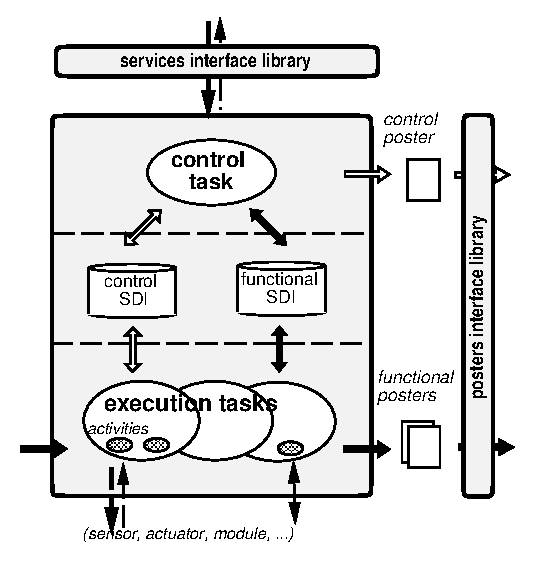
\includegraphics[width=0.5\hsize]{fig/module-en}
\caption{Structure of modules.}
\label{fig|module}
\end{figure}

\subsubsection{The control task:}

You normally do not have to care about the control task, but it's a good
idea to learn what it does. The control task

\begin{enumerate}
\item it receives the requests for the module,
\item it checks the validity of the input parameters and store them in the fIDS,
\item it checks if the module can start a given service (handles conflicts
between requests),
\item it tells the right execution task to start the service,
\item and upon the termination of a service it sends back to the client
any output produced by the service (the execution report and possibly the
C structure declared for that service).
\end{enumerate}

Beside    this, the control task  maintains   a poster  (the \emph{control
poster}) that contains informations on   the current state of the  module
(running services, activities, and so on).

Conflicts between services are   handled  according to the following  rule:  if
incompatible  services are to  be run  at the  same  time, \textbf{the last
request   has  the  priority}. Activities    that  happen to  be
incompatible  with that new request are  interrupted. This strategy matches a
\emph{reactivity} criterion and is systematically applied.

You must  declare  yourself which  services  are incompatible with  which
services. Note that   a service is  \emph{very often}  incompatible  with
itself; you must not forget to declare this.


\subsubsection{Execution tasks:}

Your own code is executed by the execution(s) task(s).

If  this code is to  be periodical (servoing,  monitoring, filters, ...),
you will have to use a periodical  execution task and specify its period.
It   is  also  possible   to use   a-periodical  tasks  and  a  sequential
scheduling. Tasks are  given priorities (supported under real-time
operating systems only),
depending on their constrains in terms of resources and CPU requirements.

In the  \texttt{demo} example,  there were  only one  execution  task 
(\texttt{exec\_task MotionTask}). 
This   is  usually  sufficient since  a   single
execution task can handle \emph{several}  activities in parallel. However,
if several  activities require different  priorities or periods, you will
have to declare several execution tasks.


\subsubsection{Interface libraries:}

Modules provide two standard interface libraries in various programming
languages (for now: \texttt{C, tcl, XML, open-prs}).

\begin{itemize}
\item A service library, which handles requests emission and reception,
\item A poster library, which contains the necessary functions to read
the module posters.
\end{itemize}


% -----------------------------------------------------------------------

\section{Integration of the algorithms: the codels}
\label{sec|module|codels}

In order to associate your code to the requests, you have to tell \GenoM\
which are the  functions that must be  executed to  handle requests. Your
algorithms must be split into several parts (startup, main function, end,
interruption, ...).   Each  of  these   parts  is called  a   \emph{codel}
(elementary code). At this time, codels are \texttt{C} functions.

A module is the result of  the link edition between  the code \GenoM\ has
generated and the codels libraries.


\chapter{Editing a module}
\label{cha|edit}
%
% Copyright (c) 2001,2009 LAAS/CNRS                        --  Tue Oct 30 2001
% All rights reserved.                                     Anthony Mallet
%
% This document is a translation of the French documentation of GenoM,
% originally written by Sara Fleury and Matthieu Herrb.
%
% Redistribution  and  use in source   and binary forms,  with or without
% modification, are permitted provided that  the following conditions are
% met:
%
%   1. Redistributions  of  source code must  retain  the above copyright
%      notice, this list of conditions and the following disclaimer.
%   2. Redistributions in binary form must  reproduce the above copyright
%      notice,  this list of  conditions and  the following disclaimer in
%      the  documentation   and/or  other  materials   provided with  the
%      distribution.
%
% THIS SOFTWARE IS PROVIDED BY THE  AUTHOR AND CONTRIBUTORS ``AS IS'' AND
% ANY  EXPRESS OR IMPLIED WARRANTIES, INCLUDING,  BUT NOT LIMITED TO, THE
% IMPLIED WARRANTIES   OF MERCHANTABILITY AND  FITNESS  FOR  A PARTICULAR
% PURPOSE ARE DISCLAIMED.  IN NO  EVENT SHALL THE AUTHOR OR  CONTRIBUTORS
% BE LIABLE FOR ANY DIRECT, INDIRECT,  INCIDENTAL, SPECIAL, EXEMPLARY, OR
% CONSEQUENTIAL DAMAGES (INCLUDING,  BUT  NOT LIMITED TO, PROCUREMENT  OF
% SUBSTITUTE  GOODS OR SERVICES;  LOSS   OF  USE,  DATA, OR PROFITS;   OR
% BUSINESS  INTERRUPTION) HOWEVER CAUSED AND  ON ANY THEORY OF LIABILITY,
% WHETHER IN CONTRACT, STRICT LIABILITY, OR TORT (INCLUDING NEGLIGENCE OR
% OTHERWISE) ARISING IN ANY WAY OUT OF THE  USE OF THIS SOFTWARE, EVEN IF
% ADVISED OF THE POSSIBILITY OF SUCH DAMAGE.
%

Creating a new module implies writing two distinct parts: the description
of the module  (the \texttt{.gen} file)  and codels. This  chapter describes
the first part, the \texttt{.gen} file.

% -----------------------------------------------------------------------
\section{Using the XEmacs mode \texttt{genom-mode}}

It is strongly advised you use the \texttt{genom-mode} under XEmacs to write
your module.  Besides the syntactic  coloring and automatic  indentation,
this   mode defines several   commands   that create  \GenoM\  structures
(requests, posters, \ldots). It also includes on-line help.

Note that for now \texttt{genom-mode} works only with \texttt{xemacs} and not anymore
with emacs...

Commands can be accessed by three means:
\begin{itemize}
\item The (X)Emacs menu bar (\texttt{GenoM Mode Commands})
\item A pop-up menu with button 3 of the mouse
\item The following keyboard shortcuts, beginning with \texttt{C-c} (control-c)

{\small
\begin{tabular}{|l|p{10cm}|}
\hline
\tt C-c C-m & create a new \underline{\textbf{m}}odule  (\emph{first command to invoke})\\
\tt C-c C-i & \underline{\textbf{i}}mport structures from another module\\
\tt C-c C-r & create a \underline{\textbf{r}}equest \\
\tt C-c C-p & create a \underline{\textbf{p}}oster \\
\tt C-c C-e & create an \underline{\textbf{e}}xecution task\\
\hline
\tt C-c C-b & indent whole \underline{\textbf{b}}uffer \\
\tt C-c C-v & \underline{\textbf{v}}erify that every field is filled \\
\tt C-c C-d & remove optional fields that are empty (\underline{\textbf{d}}elete) \\
\hline
\tt C-c C-h \ldots & on-line \underline{\textbf{h}}elp\\
\hline
\end{tabular}}
\end{itemize}

Commands that create a \GenoM\ structure (request, poster, \ldots) prompt
you  for  a   name in  the   mini-buffer.  Additional   arguments may  be
requested, depending on the particular structure you  are creating.  Once
you  have  supplied all the  arguments,  a template  for the structure is
inserted  in the buffer.   Optional   fields  are surrounded  by   single
superior and inferior signs (\texttt{$<$} and \texttt{$>$}). Mandatory  fields
are surrounded by two  superior and inferior signs  (\texttt{$<<$}  and 
\texttt{$>>$}). You  can refer to the  on-line help to know  how to fill in these
fields.

On-line help can be requested with the \texttt{C-c C-h} key sequence,
followed by one of the following letter:

{\small
\begin{tabular}{|l|p{10cm}|}
\hline
\tt h & lists the available commands of \texttt{genom-mode}  \\
\tt m & describes \underline{\textbf{m}}odules \\
\tt r & describes \underline{\textbf{r}}equests \\
\tt p & describes \underline{\textbf{p}}osters \\
\tt e & describes \underline{\textbf{e}}xecution tasks \\
\tt i & describes structures \underline{\textbf{i}}mportation \\
\tt g & describes the module \underline{\textbf{g}}eneration  \\
\tt c & describes the \underline{\textbf{c}}odels  \\
\tt C-h & help on help (this list) \\
\hline
\end{tabular}}

Help pages are made up of four parts:

\begin{itemize}
\item \texttt{What is a \ldots ?}: general description of the \GenoM\
structure
\item \texttt{How to create a \ldots ?}: how to create the structure
\item \texttt{How to instantiate the fields ?}: how to fill in the template
of the structure
\item \texttt{Examples}: some examples.
\end{itemize}

Last,  active   zones (updated  with   the sequence  \texttt{C-button2}) are
defined for each request and each codel  of the requests. When clicking
(button 2) on these zones, the file containing the corresponding codel(s)
is visited  and the point is positioned  onto the function. 

Note that if this function has not been written yet (new codel or even
request), then \texttt{genom-mode} prompts you to insert the empty template
of the codel (or all the codels of the request if you click on the request  
head-line). For this to work, the the module must be first regenerated once.

% =======================================================================
\section{Writing a module}

A  module description contains five   parts. The five section below  will
describe these parts, and use the \texttt{demo} module as an example.
The five parts are:

\begin{enumerate}
\item Module declaration
\item \texttt{C} structures and fIDS declaration
\item Requests definition
\item Posters definition
\item Execution tasks declaration
\end{enumerate}

All the  \GenoM\ structures (module,  request, poster  and task) use  the
same syntax: a keyword, which characterizes the  structure, followed by a
name and several fields enclosed between  braces (\texttt{\{} and \texttt{\}}).
The keyword is one of \texttt{module, import  from, request, poster} or 
\texttt{exec\_task}.

In this section, optional  fields are  surrounded  by \texttt{$<$} and  
\texttt{$>$}. Mandatory fields are surrounded by  \texttt{$<<$} and \texttt{$>>$}. {\em
Optional   fields that are not  instantiated  must  be removed before the
module is generated}.

% -----------------------------------------------------------------------
\subsection{Module declaration}

A module declaration looks like this:

\begin{center}\begin{cartouche}\small\begin{verbatim}
module <<module-name>> {
    number:            <<module-number>>;
    internal_data:     <<SDI-type>>;
    version:           <"version-string">;
    email:             <"address">;
    requires:          <package-dependency> , ...;
    codels_requires:   <package-dependency> , ...;
    lang:              <c or c++>;
};
\end{verbatim}\end{cartouche}\end{center}


This part   is  mandatory  and    lets   you  choose a  name   for   your
module.  Fill-in the field  \texttt{$<<$module-name$>>$}.

The parameters are the following:

\begin{itemize}
\item \texttt{number:} is the identification number of the module. 
      It must be greater that $1000$ (small numbers are reserved for
      system) and smaller than $2^{15}=32768$. It should be unique and no other
      module should use the same one. It is used to generate unique error
      report numbers.

\item \texttt{internal\_data:} is the name of  a valid \texttt{C} type.  This
      will be the module internal database (IDS). \texttt{genom-mode}
      provides you with a default value for this field.

\item \texttt{version} is a string enclosed in double-quotes that defines
      the external version number of your module. This is used by the GNU
      build tools in various places. You should incremement it before
      releasing a new version of a module. 

\item \texttt{iface\_version:} is similar but it is the \texttt{libtool}
	version of the module, not the required package. The strategy 
	relatively to the module versioning is still not well defined and
	for now this field is rarely used.

\item \texttt{email} is the contact address for the module. This will
      be copied in some files generates by the GNU build tools. Make
      sure you use an address that will be valid in the future if you
      plan to release and distribute your module.

\item \texttt{requires:} allows mainly to list the other /GenoM/ modules
      that are imply within this \texttt{.gen} file (referenced
      structures). More generally, it allows to declare the list of
      packages (in the sens of \texttt{pkg-config}) require to generate this
      \texttt{.gen} file. 

\item \texttt{codels\_requires:} it allows to declare the list of packages
	(in the sens of \texttt{pkg-config})
	require to compile and link the codels (and only the codels).

\item \texttt{lang} sets the programming language used by the
      codels. It defaults to ``C''. ``C++'' can be used to set the
      language of the codels to C++.

\end{itemize}


% -----------------------------------------------------------------------
\subsection{\texttt{C} structures and fIDS declaration}

Note:  the  \emph{functional internal  data  structure} (fIDS, or  SDIf in
French) is  a \texttt{C} structure that  contains all the requests input and
output data,  as well as the  posters definition.  When writing a module,
this structure  will  be defined  progressively  by   adding the requests
parameters each time a new request is added: do not try to write it 
\emph{a priori}.

\subsubsection{Requests parameters, replies and posters}

These are \texttt{C} structures you should define  in \texttt{C} header files.
You can include  these headers with the \texttt{\#include} directive, as in
plain \texttt{C}.  Since these headers are parts  of the  module definition,
they should be located in the main directory  of your module, in the same
place as the \texttt{.gen} file.

These structures will be used by other modules or programs.  Thus, it is
\emph{strongly} advised you prefix their names with the name of your
module to avoid conflict and determine its origin (see the example 
\texttt{demoStruct.h} in the section~\ref{sec|session|example}).

Lastly, it is also advised you protect your headers of multiple inclusion
with the standard strategy:

\begin{center}\begin{cartouche}\small\begin{verbatim}
#ifndef FILENAME
#define FILENAME
...
#endif  /* FILENAME */
\end{verbatim}\end{cartouche}\end{center}

You must respect three rules in order to get your header files working
with \GenoM:

\begin{enumerate}
\item \textbf{Allowed C types}: \GenoM\ can parse \emph{nearly} all \texttt{C}
type declarations. The  only unknown type  is \texttt{void}  and a few other
constructions are  forbidden:  \emph{i.}   \texttt{union}s,  and  \emph{ii.}
recursive type definition as   in \texttt{typedef B A}   where \texttt{A}  is a
typedef itself. A workaround for the latter is to use a new structure:

\begin{center}\begin{cartouche}\small\begin{verbatim}
typedef struct B {
   A a;
} B;
\end{verbatim}\end{cartouche}\end{center}

\item \textbf{Limitations on pointers}: Requests parameters, replies and
posters  will  travel  between  several  processes,  outside  the module,
possibly on  another machine.  Given that,  the  notion of \emph{pointer},
\emph{address} or \emph{list} does not make  sense.  They should not appear
in this context (but  you  can use  such data  types internally in   your
codels).

\item \textbf{Alignment considerations}: The structures you define can
potentially be transferred across several  platforms.  You must be  aware
that different systems do not  align data in   the same way. In order  to
avoid problems, you should  align yourself your data  on \texttt{double}s (8
bytes). The following example illustrates this:

\begin{center}\begin{cartouche}\small\begin{verbatim}
typedef struct PILO_MOVE {
   int    percentSpeed;    /* percentage of max speed */
   int    padding;         /* ALIGNMENT */
   double distance;        /* distance to travel */
} PILO_MOVE;
\end{verbatim}\end{cartouche}\end{center}

\end{enumerate}


\subsubsection{External structures}

It is  possible to   import,  from  other  modules, external    structure
definitions. The corresponding headers are included with the 
\texttt{\#include} directive but, in that case, it must be protected in an 
\texttt{import from}    directive.  This tells \GenoM\     from which module  the
structures come, and  avoid duplication of  the functions that deal  with
these structures.

It is strongly recommended that you do not hard-code the path to the
external headers. 

The field \texttt{requires:} within the module declaration structure, will
allow \GenoM\ to automatically find out the corresponding header and
library files using \texttt{pkg-config}.

It is also possibly to specify path by hand using \GenoM\ options 
\texttt{-I<path>}, \texttt{-J<VAR>=<path>} or \texttt{-P<package>} (see
chapter~\vref{cha|generation}).

In the example  below, the module  \texttt{pilo} uses  structures defined in
the module \texttt{loco}:

\begin{center}\begin{cartouche}\small\begin{verbatim}
module pilo {
     ...
     requires:    loco;
};

import from loco {
#include "locoStruct.h"
};
#include "piloStruct.h"

typedef struct PILO {
     PILO_MOVE move;
     LOCO_REF  reference;
} PILO;
\end{verbatim}\end{cartouche}\end{center}

\subsubsection{What should (and should not) the fIDS contain?}

Requests parameters, requests replies  and almost every poster  will pass
through the fIDS: thus, they must be declared in this structure. The fIDS
is also a way to   exchange data between tasks    (or threads) inside   a
module. Conversely, data exchanged between codels of  the \emph{same} task
only do not need to be declared here (but only within the codels file).


% -----------------------------------------------------------------------
\subsection{Requests definition}

There     are  threes   types of      requests:  control, execution   and
initialization. The three types are  identified  by the field \texttt{type}
and one of the three keywords \texttt{control}, \texttt{exec} and \texttt{init}.

Examples of requests can be found in the chapter~\ref{cha|session}.

\subsubsection{Control requests}

They are defined with the keyword \texttt{control} in the field \texttt{type}:

\begin{center}\begin{cartouche}\small\begin{verbatim}
request <<request-name>> {
     doc:                    <"doc">;
     type:                   control;
     input:                  <name>::<sdi-ref>;
     input_info:             <default-val>::<"name">, ...;
     output:                 <name>::<sdi-ref>;
     codel_control:          <codel-name>;
     fail_reports:           <report-name>, ... ;
     interrupt_activity:     <exec-rqst-name>, ...;
};
\end{verbatim}\end{cartouche}\end{center}

\begin{itemize}
\item \texttt{doc} is a short string that describes the service usage.

\item \texttt{input} and \texttt{output} define respectively the input
parameter and the output parameter of the request. \texttt{name} is the name
of this variable and  \texttt{sdi-ref} the name  of the corresponding member
of the fIDS (e.g. \texttt{input: position::state.position}).

\item \texttt{input\_info} lets you define default values as well as a
comment for \emph{each}   member  of  the  \texttt{input}  structure.  This
information is used for interactive  requests invocation.

\item \texttt{codel\_control} is a codel (\texttt{C} function) which is
executed by the control task and which controls the validity of the input
parameter.

\item \texttt{fail\_reports} is a list of possible reports returned by the
control codel (the special report "OK" is always implicitly defined).

\item \texttt{interrupt\_activity} is a list of requests of \emph{this module}
that   are    declared   incompatible  with     this request.  Activities
corresponding to the listed requests will  be interrupted upon invocation
of this service.  Two special keywords \texttt{all} and \texttt{none} let  you
declare all requests (or none) to be incompatible with this one.
\end{itemize}


\subsubsection{Execution requests}

They are defined with the keyword \texttt{exec} in the field \texttt{type}. As
opposed to the control requests, those requests declare services that
will be executed and they define a few more fields:

\begin{center}\begin{cartouche}\small\begin{verbatim}
request <<request-name>> {
     doc:                   <"doc">;
     type:                  exec;
     exec_task:             <<exec-task-name>>;
     input:                 <name>::<sdi-ref>;
     input_info:            <default-val>::<"name">, ...;
     output:                <name>::<sdi-ref>;
     codel_control:         <codel-name>;
     codel_start:           <codel-name>;
     codel_main:            <codel-name>;
     codel_end:             <codel-name>;
     codel_inter:           <codel-name>;
     codel_fail:            <codel-name>;
     fail_reports:          <report-name>, ... ;
     interrupt_activity:    <exec-rqst-name>, ... ;
};
\end{verbatim}\end{cartouche}\end{center}

\begin{itemize}
\item \texttt{exec\_task} is the name of the execution task in charge of the
codels execution.

\item \texttt{posters\_input:} structure types of the posters that the
execution codels of this request will read (see \S~\vref{sec|posters}).

\item \texttt{codel\_activity\_start}, \texttt{codel\_activity\_main}, 
\texttt{codel\_activity\_end},\\ \texttt{codel\_activity\_inter} and  
\texttt{codel\_activity\_fail} are the codels of this service.  All fields are
optional, but at least one of \texttt{codel\_activity\_start}, 
\texttt{codel\_activity\_main} or \texttt{codel\_activity\_end} must be defined.
Be careful that all activities can be interrupted: do not forget to
fill-in \texttt{codel\_activity\_inter} if something must be done in such a
case.
Note that \texttt{codel\_activity\_fail} is rarely used.
Codels are further described in chapter~\ref{cha|codels}.


\item All other fields serve the same purpose  as in control  requests.
See previous paragraph for a description.

\end{itemize}


\subsubsection{Initialization request}

A special execution request is the \emph{initialization request}. It is
identified by the keyword \texttt{init} in the field \texttt{type} (all other
fields are the same as for execution requests).  This special request can
be used to perform some initialization upon module startup. There can be
at most one such request and the module will not accept to serve any
other \emph{execution} request until the \texttt{init} has been invoked.
Control requests will still be served, and can be used to set several
parameters used by the \texttt{init} request.

In  order to allow the  invocation  of the init  request  from a standard
shell (for instance as soon as the  module is spawned), \GenoM\ builds an
executable called \texttt{<module>Init} (where \texttt{<module>} is the name of
the module). This executable takes exactly as
many parameters as in the structure  declared in the  input field, in the
same order as they appear in the structure.

\subsection{Posters definition}

The  posters let you export   data, either automatically  (you don't have
anything to do) or ``by hand'' inside  a codel.  Data may  be a member of
the fIDS or not.

\subsubsection{Data from the fIDS}

\begin{center}\begin{cartouche}\small\begin{verbatim}
poster <<poster-name>> {
     update:             <<update-type>>;
     data:               <<name>>::<<sdi-ref>>, ... ;
     exec_task:          <<exec-task-name>>;
};
\end{verbatim}\end{cartouche}\end{center}

\begin{itemize}
\item \texttt{update} indicates whether the poster is updated automatically
(\texttt{auto}) or by  a codel (\texttt{user}). The  \texttt{auto} mode is usually
chosen for periodical data such as a position.

\item \texttt{data} is the list of data you wish to include in the
poster. It is given in the same way as the input and output parameters of
the requests: a name, followed by a reference to a member of the fIDS.

\item \texttt{exec\_task} is the task which owns the poster. This task is in
charge of the update of the poster for \texttt{auto} posters. Note that only
the task which owns the poster can change its content.
\end{itemize}

The data  structure  of the  poster is  a concatenation  of  the  list of
declared data.  The corresponding  \texttt{C} type  is defined by \GenoM\ in
the     file   \texttt{server/<module>Poster.h} and     its    name  is  
\texttt{<MODULE>\_<POSTER>\_POSTER\_STR} (all uppercase) where \texttt{<MODULE>} is the name
of the module and \texttt{<POSTER>} the name of the poster.

For  instance,   the \texttt{Mobile}  poster  of    the \texttt{demo}  module
(chapter~\ref{cha|session}) is defined as follow:

\begin{center}\begin{cartouche}\small\begin{verbatim}
typedef struct DEMO_MOBILE_POSTER_STR {
  DEMO_STATE_POSTER_STR state;
  double ref;
} DEMO_MOBILE_POSTER_STR;
\end{verbatim}\end{cartouche}\end{center}


\subsubsection{Other data}

Data exported by posters  are not necessarily members  of the fIDS.  This
can be the case if \emph{i.} data structures are big: it is not advised to
put  them in   the fIDS and   copy them  several times, \emph{ii.}  data
structures do not have a predefined size, as for lists for instance.

For this kind of posters, two new fields are defined:

\begin{center}\begin{cartouche}\small\begin{verbatim}
poster <<poster-name>> {
     update:               user;
     type:                 <<name>>::<<type-name>>, ...;
     exec_task:            <<exec-task-name>>; 
     codel_poster_create:  <codel>;
};
\end{verbatim}\end{cartouche}\end{center}

\begin{itemize}
\item \texttt{type} is the name of the \texttt{C} type of the data structure.
\item \texttt{codel\_poster\_create} optionally designates the name of a \texttt{C}
function which is   used to create the  poster  structure. If  it is  not
given,  the  module performs the memory  allocation  by itself, using the
size of the  given \texttt{C} type.
\end{itemize}


\subsection{Execution tasks declaration}

\begin{center}\begin{cartouche}\small\begin{verbatim}
exec_task <<exec-task-name>> {
     period:             <number>;
     delay:              <number>;
     priority:           <<number>>;
     stack_size:         <<number>>;
     codel_task_start:   <codel>;
     codel_task_end:     <codel>;
     codel_task_main:    <codel>;
     codel_task_main2:   <codel>;
     posters_input:      <poster-type>, ...;
     error_reports:      <report-name>, ... ;
};
\end{verbatim}%
\end{cartouche}\end{center}

\begin{itemize}
\item \texttt{period} (optional) defines a periodical task. The period is
given as an integer number in \texttt{ticks} (at the moment, a tick is $5ms$
under VxWorks and $10ms$ under Unix). \emph{Remark:} previously the period was to be 
\emph{a divisor or a multiple} of $20$. (e.g. 1, 2, 4, 5, 10, 20, 40, 60,
\ldots. This constraint has been raised.

\item \texttt{delay} (optional integer in \emph{ticks}). All periodical
tasks with the same period  will wake up at the  same time. The delay can
be used to delay the waking up of a particular task  by the amount of ticks 
specified. \texttt{delay} can be \texttt{none} for  a-periodical tasks. Pertinent only on real-time OS.

\item \texttt{priority} is used by the scheduler of the operating system. It
is an integer  between $0$ (highest) and  $255$ (lowest). Priorities must
be used to make  sure that tasks  with strong real-time constraints  will
match their requirements.  A common strategy is to use a priority roughly
``proportional to the inverse'' of the period. Pertinent only on real-time OS.

\item \texttt{stack\_size} is the size (in bytes) of the stack for this
task. The size you  need  depends essentially on   the size of the  local
variables you  use.  A   stack which  is \emph{too small} will   produce
unpredictable results, so be sure  to largely \textbf{overestimate} what you
need.   A  good choice is  usually   $20.000$  bytes. Note that under
Unix, stack size are not used at this time (the stack is grown dynamically).  Pertinent only on real-time OS.

\item \texttt{codel\_task\_start} is the initialization codel. It is called only
once, just before the module is ready to answer requests.  It can be used
to initialize internal variables (see also  the \emph{init request}, which
can be used if the initialization requires user inputs).

\item \texttt{codel\_task\_end} is the symmetric of the \texttt{codel\_task\_start}. It
is called once, just before the module exits.

\item \texttt{codel\_task\_main} is a \emph{permanent} codel. It is executed each time
the execution tasks wakes  up (\emph{before} all the other activites). Thus, for  a  periodical task, it is  also
periodical.

\item \texttt{codel\_task\_main2} is a \emph{permanent} codel. It is executed each time
the execution tasks wakes  up (\emph{after} all the other activites). Thus, for  a  periodical task, it is  also
periodical.

\item \texttt{posters\_input:} structure types of the posters that the
execution codels of this task will read (see \S~\vref{sec|posters}).

\item \texttt{error\_reports} is a list of reports that can be reported by the
permanent activity \texttt{codel\_task\_main}. Since  this activity does not belong to
a request, its  reports are  stored in  the  \emph{control poster} of  the
module.
\end{itemize}


\chapter{Module generation}
\label{cha|generation}
%
% Copyright (c) 2001 LAAS/CNRS                        --  Wed Oct 31 2001
% All rights reserved.                                     Anthony Mallet
%
% This document is a translation of the French documentation of GenoM,
% originally written by Sara Fleury and Matthieu Herrb.
%
% Redistribution  and  use in source   and binary forms,  with or without
% modification, are permitted provided that  the following conditions are
% met:
%
%   1. Redistributions  of  source code must  retain  the above copyright
%      notice, this list of conditions and the following disclaimer.
%   2. Redistributions in binary form must  reproduce the above copyright
%      notice,  this list of  conditions and  the following disclaimer in
%      the  documentation   and/or  other  materials   provided with  the
%      distribution.
%
% THIS SOFTWARE IS PROVIDED BY THE  AUTHOR AND CONTRIBUTORS ``AS IS'' AND
% ANY  EXPRESS OR IMPLIED WARRANTIES, INCLUDING,  BUT NOT LIMITED TO, THE
% IMPLIED WARRANTIES   OF MERCHANTABILITY AND  FITNESS  FOR  A PARTICULAR
% PURPOSE ARE DISCLAIMED.  IN NO  EVENT SHALL THE AUTHOR OR  CONTRIBUTORS
% BE LIABLE FOR ANY DIRECT, INDIRECT,  INCIDENTAL, SPECIAL, EXEMPLARY, OR
% CONSEQUENTIAL DAMAGES (INCLUDING,  BUT  NOT LIMITED TO, PROCUREMENT  OF
% SUBSTITUTE  GOODS OR SERVICES;  LOSS   OF  USE,  DATA, OR PROFITS;   OR
% BUSINESS  INTERRUPTION) HOWEVER CAUSED AND  ON ANY THEORY OF LIABILITY,
% WHETHER IN CONTRACT, STRICT LIABILITY, OR TORT (INCLUDING NEGLIGENCE OR
% OTHERWISE) ARISING IN ANY WAY OUT OF THE  USE OF THIS SOFTWARE, EVEN IF
% ADVISED OF THE POSSIBILITY OF SUCH DAMAGE.
%
% $Id$
%

% =======================================================================
\section{The {\tt genom} command}

\begin{description}

\item{\bf Synopsis}

{\tt genom [-Ocdintx] [-I{\em path}] [-D{\em macro}] <module>[.gen]}

\item{\bf Description}

{\tt genom}  is the  command that  generates a  module. The  {\tt module}
argument is the name  of the file which  contains the description of  the
module. The {\tt  .gen} is   optional and  is  automatically appended  if
omitted.

{\tt genom} accepts the following options:

\begin{tabularx}{\linewidth}{lX}
{\tt -O} & {\em Accept \textbf{O}bsolete syntax:} the syntax of
\texttt{.gen} files has changed a bit over time. This option tells
genom to still accept input syntax that is now considered as obsolete.
Warning: this option can produce output code that is incompatible with
what is generated without it. Use at your own risk. \\

{\tt -i} &  {\em Installs the  directory  {\tt codels/}:} you should  use
this option when  generating the module  for the first time. When  called
with {\tt -i}, {\tt  genom} will install  the directory {\tt  codels/} as
well as templates for  the codel files in this  directory.  It  will also
create  all the {\tt Makefiles}  (in the main directory   and in the {\tt
codels} directory) used to compile  the module.  If  the files that would
normally be  installed  are already present, {\tt   genom}  will ask  for
confirmation before overwriting files.\\

{\tt -c} & {\em Conditional regeneration:} module is regenerated only
if files from which  it depends have  been modified since last generation
({\em i.e.} the {\tt .gen} file or files it includes).\\

{\tt -t} &    {\em Tcl libraries  generation:}    Generates Tcl interface
libraries. They are mandatory  if you wish to  control this module from a
tcl interpreter (see section~\ref{sec|tcl}).\\

{\tt    -x}  & {\em    Propice   libraries generation:} Generates Propice
interface libraries.  They are  mandatory  if you   wish to  control this
module from a Propice program.\\

{\tt -n} & Generates the perl script that is used to generate the module,
without actually executing it.\\

{\tt -d} & Turns on debugging mode inside the {\em yacc} parser.\\

{\tt -I{\em path}} & Defines paths for included files (same as {\tt
-I} option of {\tt cc}).\\

{\tt -D{\em macro}} & Defines macros as for {\tt cc}.\\
\end{tabularx}

Once the module has been installed ({\tt -i} option)  for the first time,
you just   have to invoke {\tt make}   (GNUmake is required)  in the main
directory to regenerate or compile the module.

The {\tt -i} option modifies files in the {\tt codels/} directory. Use it
carefully.  If you wish  to manually  get a  new   template file for  the
codels, you can find them in the directory {\tt .genom/codels/}.  These files
are always  up-to-date. Also consider the  XEmacs  mode {\tt genom-mode},
which lets  you  insert codel templates  into  existing codel files  (see
chapter~\ref{cha|edit}).

\end{description}


% =======================================================================
\section{Product of the generation}

The module generation produces files in the two directories {\tt codels/}
and {\tt server/}.  The files located  in the  {\tt codels/}  directory are
described in the next chapter.  This  section describes the files located
in  the  {\tt server/} directory.   The {\tt  demo} module   is  used as an
example: you can always replace the string {\tt demo} by the name of your
module.

Compiling these files produces binary objects and executables in the {\tt
\$\{TARGET\}} sub-\-directories. See appendix~\ref{anx|files} for
information on the file-system hierarchy.

% -----------------------------------------------------------------------
\subsection{Interface libraries}

\subsubsection{Requests library: {\tt demoMsgLib}}

This library implements  the basic requests  functions (request emission,
replies reception) and is used by the clients of this module.

The {\tt   C}  source code    of  this  library  can be   found  in  {\tt
demoMsgLib.c}.  The header
file {\tt demoMsgLib.h}, which must  be included by clients, contains the
definitions for the server identification and communication establishment
(name and size of the mailbox, function prototypes\ldots).

To use this  library, you must link your  program with  {\tt
-ldemoClient}. 


\subsubsection{Posters library: {\tt demoPosterLib}}

This library implements the basic posters functions for this module (read
and display   functions).  The same    structure as above  is used:  {\tt
demoPosterLib.c} is  the  source code. 
{\tt demoPosterLib.h}   defines the name  of  the
posters along  with  their data structures and prototypes of access
funtions.
The  {\em cIDS} structure is
also defined there\footnote{the structures included by the {\em cIDS} are
defined in the file {\tt modules.h}, located in the genom source tree.}.

To  use this library,  you must link  with  {\tt 
-ldemoClient}.


% -----------------------------------------------------------------------
\subsection{Useful header files}

The file {\tt  demoHeader.h} must  be included  in every  codel file.  It
contains the definitions of several constants that characterize the module
(name, period, posters, \ldots)  as well as the two  macros that let  you
access the {\em IDS} ({\em SDI\_F} and {\em SDI\_C}).

The file  {\tt demoError.h} contains the  definitions of the  error codes
(reports declared in the {\tt fail\_reports} field) of this module.

The file {\tt  demoType.h} defines the actual {\em  IDS} structure. It is
not necessarily the same as  in the  {\tt .gen}  file, especially if  the
module   defines   reentrant   requests   ({\em  i.e.}   compatible  with
themselves).

% -----------------------------------------------------------------------
\subsection{Tcl library}

The files  {\tt demoTcl.c} and {\tt demo.tcl}  are used by Tcl to control
the module. See section~\ref{sec|tcl} in this document.


% -----------------------------------------------------------------------
\subsection{Propice library}

The files located in the {\tt propice/} directory are  used by Propice to
control the module. See section~\ref{sec|propice} in this document.


% -----------------------------------------------------------------------
\subsection{Executables: server, test program, initialization request}

The executable {\tt demoTest} is an interactive test program. To use it,
you just have to  run
{\tt \$\{TARGET\}/demoTest}.

The  files    {\tt demoCntrlTask.c},   {\tt demoMotionTask.c}    and {\tt
demoModuleInit.c} contain the module's execution tasks source code.  Once
compiled, they produce the  files  {\tt
libdemoServer.a}.  The   file  {\tt demoModuleInit.c} produces    the
function {\tt demoTaskInit} which spawns the module.

The file {\tt demoInit.c} contains the code that invokes the {\em
Initialization} request of the module (if the module defines one). To use
it, run {\tt demoInit} (the executable is in {\tt
\$\{prefix\}/bin}.


% -----------------------------------------------------------------------
\subsection{Other files}

The  files {\tt demoScan.h} and {\tt  demoPrint.h} contain the definition
of  the interactive   functions  that scan  the  arguments  of the module
requests. These functions are used by the test program {\tt demoTest}.

Appendix~\ref{anx|files} gives an exhaustive list  of the files  produced
by \GenoM.


\chapter{Writing the codels}
\label{cha|codels}
%
% Copyright (c) 2001 LAAS/CNRS                        --  Sat Nov  3 2001
% All rights reserved.                                     Anthony Mallet
%
% This document is a translation of the French documentation of GenoM,
% originally written by Sara Fleury and Matthieu Herrb.
%
% Redistribution  and  use in source   and binary forms,  with or without
% modification, are permitted provided that  the following conditions are
% met:
%
%   1. Redistributions  of  source code must  retain  the above copyright
%      notice, this list of conditions and the following disclaimer.
%   2. Redistributions in binary form must  reproduce the above copyright
%      notice,  this list of  conditions and  the following disclaimer in
%      the  documentation   and/or  other  materials   provided with  the
%      distribution.
%
% THIS SOFTWARE IS PROVIDED BY THE  AUTHOR AND CONTRIBUTORS ``AS IS'' AND
% ANY  EXPRESS OR IMPLIED WARRANTIES, INCLUDING,  BUT NOT LIMITED TO, THE
% IMPLIED WARRANTIES   OF MERCHANTABILITY AND  FITNESS  FOR  A PARTICULAR
% PURPOSE ARE DISCLAIMED.  IN NO  EVENT SHALL THE AUTHOR OR  CONTRIBUTORS
% BE LIABLE FOR ANY DIRECT, INDIRECT,  INCIDENTAL, SPECIAL, EXEMPLARY, OR
% CONSEQUENTIAL DAMAGES (INCLUDING,  BUT  NOT LIMITED TO, PROCUREMENT  OF
% SUBSTITUTE  GOODS OR SERVICES;  LOSS   OF  USE,  DATA, OR PROFITS;   OR
% BUSINESS  INTERRUPTION) HOWEVER CAUSED AND  ON ANY THEORY OF LIABILITY,
% WHETHER IN CONTRACT, STRICT LIABILITY, OR TORT (INCLUDING NEGLIGENCE OR
% OTHERWISE) ARISING IN ANY WAY OUT OF THE  USE OF THIS SOFTWARE, EVEN IF
% ADVISED OF THE POSSIBILITY OF SUCH DAMAGE.
%
% $Id$
%

Codels are {\tt C} functions (at this time) that interface a module and
your algorithms: the module executes the codels, which, in turn, execute
your   own functions. In   particular,  codels can retrieve  the requests
parameters,  map them into useful data  for your functions, and then call
these functions.

% =======================================================================
\section{Different kinds of codels}

% -----------------------------------------------------------------------
\subsection{Codels associated to requests}

Sending a request to a module ends up in executing the code of the codels
associated to the request. Two types of codels can be distinguished:

\begin{itemize}
\item {\bf control codels} (defined with {\tt c\_control\_func}) are
executed by the control task. They are essentially  used for checking the
validity    of the input parameters of    the  request, just before these
parameters are actually written into the fIDS.

\item {\bf execution codels} (defined with {\tt c\_exec\_func*}) are
executed by  an execution task  and  represent the actual  action of  the
service.    Their execution  create   an  activity,   which lasts   until
completion  of  the service.   These  codels  exist   only for  execution
requests.
\end{itemize}

The parameters of the {\tt C} functions associated to  the codels are the
{\tt  input} and {\tt output} structures  of  the request. The input data
can thus be passed to your functions, and you can  write the results into
the output structure.


% -----------------------------------------------------------------------
\subsection{Codels associated to execution tasks}

Three codels can be optionally defined for each execution task:

\begin{itemize}
\item {\bf Initialization codel} ({\tt c\_init\_func}). This codel is
executed  only once, when  the  execution task   is initialized and  just
before it starts serving requests.  One can use  this codel to initialize
the fIDS, and set default values to parameters.

\item {\bf Termination codel} ({\tt c\_end\_func}). This codel is
executed by the execution task upon destruction of the module, just after
it has stopped serving requests.

\item {\bf Permanent codel} ({\tt c\_func}). This codel is executed
each  time  the task  wakes  up (therefore  periodically  if  the task is
periodic). This codel creates a permanent activity.
\end{itemize}


% =======================================================================
\section{Simple examples of codels}

% -----------------------------------------------------------------------
\subsection{Example of control codel}
\label{ssec|control|ex}

Control codels are used  to check the  validity of input parameters  of a
control  or  an execution request.    They can prevent entering erroneous
values  into the fIDS. For execution  requests, they can  also check that
the  module  is in   an adequate  state before  executing  the  requested
service.

Control codels take the input parameter of the  request as input and must
return either {\tt OK} if the parameter is valid, or {\tt ERROR} if it is
not. Warning: in the latter case, you must have defined an error code and
you must set it before returning {\tt ERROR}.

If the  codel returns {\tt  OK}, the  input parameter  is copied into the
fIDS and the execution  continues. If the  codel returns {\tt ERROR}, the
parameter is not copied into the fIDS and the final reply is sent back to
the client, along with the report which has been set by the codel. For an
execution  request,  the  activity is  not  started.   The error code  is
fundamental: if it is  not  set, the client   will have no idea  of  what
happened.

As an example, here  is the control  codel {\tt demoControlSpeed} of  the
request {\tt SetSpeed} of the module {\tt  demo}.  This request expects a
speed as input (structure {\tt DEMO\_SPEED}).  Therefore, the codel takes
a pointer   to  this structure as  first  parameter.   The structure {\tt
DEMO\_STR}  is   defined    in  the    file  {\tt   demoStruct.h}    (see
chapter~\ref{cha|session}).

\begin{center}\begin{cartouche}\small\begin{verbatim}
STATUS
demoControlSpeed(DEMO_SPEED *speed, int *report)
{
   /* Refuse *speed if the value is erroneous */
   if (*speed != DEMO_SLOW && *speed != DEMO_FAST) {
        *report = S_demo_INVALID_PARAMETER;
        return ERROR;
   }
   /* Parameter is valid: it will be entered into the fIDS */
   return OK;
}
\end{verbatim}\end{cartouche}\end{center}

% -----------------------------------------------------------------------
\subsection{Example of execution codel}

Execution  codels are always associated  to   an execution request.  They
perform the actual actions of the service.

For this first example, we will write a request  that compute the norm of
a 2-dimensional vector. The standard math library already has such a
function:

\begin{center}\begin{cartouche}\small\begin{verbatim}
double
hypot(double x, double y);
\end{verbatim}\end{cartouche}\end{center}

What we have to do now  is to add  to the module  a request which we call
{\em Hypot}. An execution codel will do  the actual computation, and call
{\tt hypot()}. The input parameter will be a structure which will contain
two members, {\tt x} and {\tt y}: we call it {\tt DEMO\_VECTOR\_STR}. The
output parameter is a single {\em double}.

In the file {\tt demo.gen}, we write:

\begin{center}\begin{cartouche}\small\begin{verbatim}
/* fIDS declaration */
typedef struct DEMO_STR {
   DEMO_STATE_STR     state;           /* Current state */
   DEMO_SPEED         speedRef;        /* Speed reference */
   DEMO_VECTOR_STR    vector;
   double             norm;
   ...
};

/* Hypot request */
request Hypot {
   doc:                 "compute sqrt(x*x+y*y)";
   type:                exec;                  /* execution request */

   input:               vector::vector;        /* vector (x, y) */
   input_info:                                 /* default values and */
      0.0::"X coordinate",                     /* description of */
      0.0::"Y coordinate";                     /* parameters */
   
   output:              norm::norm;            /* norm (result) */
   c_exec_func:         demoHypotExec;         /* execution codel */
   exec_task:           MotionTask;            /* execution task */
   incompatible_with:   Hypot;                 /* incompatibilities */
};
\end{verbatim}\end{cartouche}\end{center}

In the file {\tt demoMotionTaskCodels.c}, which contains all the codels
for this task, we write the {\tt demoHypotExec} codel:

\begin{center}\begin{cartouche}\small\begin{verbatim}
ACTIVITY_EVENT
demoHypotExec(DEMO_VECTOR_STR *vector, double *norm, int *report)
{
   *norm = hypot(vecteur->x, vecteur->y);
   return ETHER;
}
\end{verbatim}\end{cartouche}\end{center}

The {\tt  return  ETHER} statement tells   \GenoM\ that  the  activity is
terminated: the client will  get the final  reply. We will see  later the
other values that can be returned at the end of an execution codel.

The next  step is to  compile the   module,  and link   it with the  {\tt
hypot()} function.  In  this  case, {\tt  hypot} is   a function of   the
standard library, so there's nothing special  to do.  But it the function
were a function of your own, defined in a non-standard library, you would
have to edit the Makefiles and complete the variables:

\begin{itemize}
\item {\tt CPPFLAGS} for the path to the headers of your library.
\item {\tt LIBS} for the path to the library itself.
\end{itemize}

Here is what it could look like with our example and the Makefile in the
{\tt codels/} directory:

\begin{center}\begin{cartouche}\small\begin{verbatim}
[...]
CPPFLAGS += -I$(DEMO) -I$(DEMO)/auto -I$(DIRUNIX)  -I$(DIRGENOM)
CPPFLAGS += -I/usr/include
[...]
LIBS = /usr/lib/libm.a
\end{verbatim}\end{cartouche}\end{center}
%$

If your external functions  were defined in a  {\tt C}  file in the  {\tt
codel/} directory (instead of  in an external  library), you would simply
add this file to the   list  of files to  be   compiled into the   codels
library:

\begin{center}\begin{cartouche}\small\begin{verbatim}
[...]
SRCS = \
        demoCntrlTaskCodels.c \
        demoMotionTaskCodels.c
SRCS += hypot.c
[...]
\end{verbatim}\end{cartouche}\end{center}

This simple example showed how to integrate  your algorithms into codels.
The sections~\ref{sec|codels|split} page~\pageref{sec|codels|split} and
\ref{sec|codels|writing} page~\pageref{sec|codels|writing} will present
more complex examples.


% =======================================================================
\section{Codel files and compilation}

\subsection{Splitting codels into several files}

To help you   write the  codels, the {\tt   -i}  option of  {\tt   genom}
generates empty templates in the {\tt  codels/} directory. Then, you just
have to complete the templates.

{\em Note}  that if you use the  {\tt -i} option  and those files already
exist, {\tt genom} asks for confirmation before  overwriting any file. It
is not possible to  fuse locally modified  templates with fresh new ones.
However, the   templates are always generated  in  the  {\tt auto/users/}
directory, so  that  you can fuse   parts together by  yourself. The {\tt
genom-mode} can help you to do this: see chapter~\ref{cha|edit}.

By default, there is one codel file per task.  Control codels are grouped
in the  source file  {\tt demoCntrlTaskFunc.c}  and execution  codels are
grouped  in the the source  file {\tt demo<Exec  Task>Func.c}, where {\tt
<Exec Task>} is the name of the execution task for those codels.

You are    free  to define   additional  files,  or  change  the  initial
organization.  Be sure you update the  {\tt SRC} variable in the Makefile
to reflect your changes.


\subsection{Makefiles}

Several {\tt  Makefile} are generated   by {\tt genom}.  By default, they
compile your codels  files, and perform the  link edition with the module
server ({\tt demoModule.o} for VxWorks and {\tt demoServer.a} for Unix).

Each file  is compiled in the {\tt  \$\{TARGET\}} subdirectory. For unix,
the compilation  produces the executable {\tt demo}  and for  VxWorks the
object file {\tt demo.o}.

You can change the standard Makefiles to suit your needs. In particular,
you can:

\begin{itemize}
\item add files to the {\tt SRC} list.
\item add libraries to the {\tt LIBS} list.
\item add compilation flags such as {\tt -I} or {\tt -D} to the  variable
{\tt CPPFLAGS}.
\end{itemize}


% =======================================================================
\section{Accessing the IDS}

You can access   this  structure from a  codel  at  any time.   A  mutual
exclusion lock protects the structure against concurrent accesses.

\subsection{The fIDS}

The macro {\tt SDI\_F}  defined in the {\tt auto/<module>Header.h} header
represent a pointer to the fIDS of the module.

{\em Warning:} the   {\tt input}  and {\tt   output} parameters  of   the
requests  can  be those  of simultaneous activities  (if  the  request is
compatible with  itself).  In that case, these  parameters {\em  are not}
pointers to members of  the fIDS structure declared in  the module.  Each
activity  must have  its own  set  of  parameters, and \GenoM\  generates
arrays for that case. The member you have defined in the {\em fIDS} still
exists, but is not used. Thus, you should always avoid reading parameters
of  a  request  directly  from the  fIDS,  except    if that request   is
incompatible with itself.


\subsection{The cIDS}

The cIDS contains various parameters of the module (period, poster names,
clients ids, \ldots) and its current  state (activities, \ldots). You can
read  the members  of this  structure thanks   to macros  defined in {\tt
auto/<module>Header.h}.

Here is a non-exhaustive list, for a module {\tt  pilo} client of another
module {\tt loco} and with an execution task {\tt Motion} which updates a
poster {\tt Ref}:

\bigbreak

{\small\begin{tabularx}{0.8\linewidth}{|l|X|}
\hline
name & value\\
\hline
\tt PILO\_MOTIONTASK\_NUM    & Id of the exec. task {\tt MotionTask}\\
\tt PILO\_REF\_POSTER\_ID    & Poster {\tt Ref} Id\\
\tt PILO\_MOTION\_LOCO\_CLIENT\_ID & Client id for {\tt loco}\\
\tt CURRENT\_ACTIVITY\_NUM($i^*$) & Current activity number\\
\tt EXEC\_TASK\_PERIOD($i^*$) & Execution task period (seconds)\\
\hline
\end{tabularx}}

($*$)  $i$ is   the  id  of  the    execution  task, for   instance  {\tt
PILO\_MOTIONTASK\_NUM}.


% =======================================================================
\section{Reports}

In real situations, every action can fail. On a machine which
interacts with  its environment, it is {\em  necessary} to think of every
such abnormal situation, in order to protect the whole system. In case of
an execution error,  it  is necessary to {\em   i.} restore a sane  state
locally, to be able to restart another  execution and {\em ii.}  report a
precise information   to the  client so  that   it can   take appropriate
decisions.

The list of abnormal situations is defined with the field {\tt fail\_msg}
of every   request.  These   are strings,   wich are   meant to be  human
readable:       for      instance  {\tt      INVALID\_PARAMETERS},   {\tt
POSTER\_NOT\_FOUND}, {\tt NOT\_ENOUGH\_MEMORY},   {\tt IMPORTANT\_DRIFT},
{\tt CASE\_NOT\_MANAGED},\\ {\tt SOLUTION\_NOT\_FOUND}, \ldots

Reports must be precise:  avoid strings such  as {\tt ERROR}. However, it
is not necessary to recall the name  of the request:  the client knows it
already.  Thus, a  report {\tt  INVALID\_PARAMETERS}   could be used  for
several requests without loss of information.

Modules must  also   restore  themselves into  a  sane  state  and handle
correctly future   requests.   For  instance, in  the   case  of  a  {\tt
NOT\_ENOUGH\_MEMORY}, the module should free every unused memory in order
to be able to process  less demanding requests.  If  the failure is  such
that the module cannot restore a sane sate, it should put itself into the
{\tt ZOMBIE} state and wait for a human debugger.


\subsection{Numerical values of reports}

Reports which  are declared in the {\tt  fail\_msg} field are mapped into
32 bits integers with the VxWorks format.

The name of this integer is build as follow: {\tt S\_<source>\_<report>},
where {\tt <source>} is the name of the module or the library which defines
the      {\tt       <report>}     string.    For       instance:     {\tt
S\_demo\_INVALID\_PARAMETER}.

The numerical value is computed as follow:
\begin{itemize}
\item the 16 highest significative bits encode the id of the task or
the  library which  defines the report.   This  number is  the  id of the
module  $N$, $N+1$   for  the requests  library, $N+2$  for   the posters
library, $N+3$ for the first execution task, \ldots.

\item the 16 lowest significative bits encode the id of the report
inside the module, and is computed by \GenoM.
\end{itemize}

Error codes are stored in the file {\tt auto/<module>Error.h}.


\subsection{Installing the reports}

{\bf Warning: this procedure might be deprecated}.

By default, clients  will  display the  numerical value of  the  reports.
However, it is  possible to install  reports in a global database. Client
can then display  reports as human  readable strings. To  do so, you must
use  the command  {\tt    h2addErrno}  located in   the   directory  {\tt
/usr/local/hilare2/src/errorLib}:

\begin{center}\begin{cartouche}\small\begin{verbatim}
pif[demo]  cd /usr/local/robots/posix/src/errorLib
pif[errorLib] h2addErrno /usr/local/hilare2/src/modules/demo/auto/demoError.h
pif[errorLib] gnumake
\end{verbatim}\end{cartouche}\end{center}


\subsection{Displaying the reports}

{\bf Warning: this procedure might be deprecated}.

To  display a  report  in clear text,  use  function of  the library {\tt
h2errorLib} (installed in {\tt /usr/local/hilare2/src/errorLib/}).

\begin{center}\begin{tabularx}{\linewidth}{|lX|}
\hline
\tt void h2printErrno(int bilan); & display the string associated to the
report \\
\hline
\tt char const *h2getMsgErrno(int numErr); & return the string associated
to the report \\
\hline
\tt void h2perror(char *string);  & display the string {\tt string}
followed by the  the string associated to  the  last report ({\tt  errno}
variable)\\
\hline
\end{tabularx}\end{center}


% =======================================================================
\section{Updating posters}

Posters which are  declared as {\tt user}  must be updated by the codels.
There are several ways to do so: depending on the type of poster, you can
use  functions of    the      poster  library {\tt   posterLib}      (see
appendix~\ref{anx|posters}) or   the function  generated by \GenoM\  (see
below).  The function {\tt posterWrite} is of particular interrest:

\bigbreak
{\tt int posterWrite(POSTER\_ID posterId, int offset, char *buf, int nbytes)}
\bigbreak

{\tt posterId} is the poster id: e.g. {\tt PILO\_REF\_POSTER\_ID} for the
poster {\tt Ref} in  module {\tt  pilo}.   {\tt posterWrite} writes  {\tt
nbytes} from buffer {\tt buf} in the poster structure, starting at offset
{\tt offset}.  It returns the  number of bytes actually written, normally
{\tt nbytes}.

\bigbreak

Consider the example  of poster {\tt   Mobile} in module {\tt  demo}. Its
structure is:

\begin{center}\begin{cartouche}\small\begin{verbatim}
typedef struct DEMO_MOBILE_POSTER_STR {
  DEMO_STATE_STR state;
  double ref;
} DEMO_MOBILE_POSTER_STR;
\end{verbatim}\end{cartouche}\end{center}
\label{typedef|demomobile}

Example 1: you update the {\tt ref} member. Since it is not at the
beginning of the poster, you must compute the offset:

\begin{center}\begin{cartouche}\small\begin{verbatim}
   DEMO_MOBILE_POSTER_STR *mobile;
   int offset;
   double ref;
   ...
   offset = (char *)(&mobile->ref) - (char *)(&mobile);
   posterWrite(DEMO_MOBILE_POSTER_ID, offset, &ref, sizeof(ref));
\end{verbatim}\end{cartouche}\end{center}

Example 2:  \GenoM\ produces a  function that  do the  same as  the above
example:

\begin{center}\begin{cartouche}\small\begin{verbatim}
   double ref;
   ...
   if (demoMobileRefPosterWrite(DEMO_MOBILE_POSTER_ID, &ref) == ERROR) {
        /* stop ... */
   }
   ...
\end{verbatim}\end{cartouche}\end{center}

\bigbreak

Another more practical  method consists in getting  the actual address of
the poster   structure.   This is done thanks    to the  {\tt posterAddr}
function. This function returns a pointer to the structure of the poster,
and you can  write into it directly. Be  sure to protect writings to  the
poster with {\tt posterTake} before    writing anything in it and    {\tt
posterGive} once you are done.

The three functions take one  parameter: the poster id. {\tt posterTake}
takes another  argument:  {\tt POSTER\_WRITE} or  {\tt POSTER\_READ}, for
accessing the poster in write or read mode.

\begin{center}\begin{cartouche}\small\begin{verbatim}
    static DEMO_STATE_POSTER_STR *addrPosterMotion = NULL;

    /* Get the poster address */
    addrPosterMotion = posterAddr(DEMO_STATE_POSTER_ID);
    if (addrPosterMotion == NULL) {
       *report = errnoGet();
       return ERROR;
    }

    /* Update the poster */
    posterTake(DEMO_STATE_POSTER_ID, POSTER_WRITE);
    addrPosterMotion->state.speed = state.speed;
    posterGive(DEMO_STATE_POSTER_ID);
\end{verbatim}\end{cartouche}\end{center}


% =======================================================================
\section{Splitting algorithms into codels}
\label{sec|codels|split}

As   we have   already  mentioned,  algorithms   must  be integrated into
codels. In the simple example presented  in the beginning of the chapter,
the  {\tt hypot} function  was put in a   single codel.  For more complex
algorithms, it will be necessary to split the functions call into several
codels. You will have to write the succession of codel calls.

The choice  of the number of  codels is generally  not unique.  But it is
important to keep in mind that a codel  is the {\em smallest} entity that
a module can handle. In particular, a  codel cannot be {\em interrupted}:
during  its execution the   module cannot do   anything else. The way you
split your algorithms will thus determine the latency of the module.

Consider  the two most  common classes of   codels: periodical codels and
aperiodical codels.

\subsection{Periodical codels}

For periodical codels (servoing, monitoring, filtering, \ldots), the same
function must be called periodically. To do so, an execution request will
be associated  to  a periodical  execution task  and  the  codel will  be
invoked at each period.

Typically, this codel  will be the {\em  execution codel} of the  request
({\tt  c\_exec\_func}).  To let   the    execution task call   the  codel
periodically, the latter must let the task know that  the activity is not
finished  when the codel  returns.  This is done  by returning {\tt EXEC}
instead  of {\tt ETHER}.  The activity stays  in the state {\tt EXEC} and
the execution codel will be called at the next task's wake up.

Consider request {\tt Monitor},   which monitorates the position   of the
mobile and  throw an  alert when it   has the requested value, say,  {\tt
myPos}.  The  execution codel  {\tt  demoMonitor} (see below)  is invoked
({\tt return EXEC;}) until the position {\tt myPos}  has not been reached
with the {\tt DEMO\_THRESHOLD} precision. Once  this position is reached,
the activity ends ({\tt return  ETHER;}) and the  final reply is sent  to
the client.

\begin{center}\begin{cartouche}\small\begin{verbatim}
ACTIVITY_EVENT
demoMonitor(double *monPos, double *pos, int *bilan)
{
   /* Get the current position */
   *pos = SDI_F->state.position;

   /* Test if we are in the monitored zone */
   if (fabs(*monPos - *pos) > DEMO_THRESHOLD) {

      /* if not, we continue with the same codel */
      return EXEC;
   }

   /* The mobile is in the goal area: end the activity */
   return ETHER;
}
\end{verbatim}\end{cartouche}\end{center}

In this example,   we used only  one execution  codel, which  was invoked
periodically.

If an algorithm had required an  initialization step (e.g.  for a sensor,
a variable, starting another service, \ldots), this  would have been done
thanks to the {\em start} codel ({\tt c\_exec\_func\_start}).  This codel
corresponds to the {\tt START} state, and  is always executed first if it
is  defined. At the  end  of this codel,  we  would {\tt return EXEC;} to
switch to  the {\tt  EXEC} state, or   {\tt ETHER} if   we  want to  stop
everything.

Similarily, a termination phasis   would be defined   thanks to the  {\em
termination codel} (the {\tt c\_exec\_func\_end} field) associated to the
{\tt END} state. To indicate, at the end of  the execution codel, that we
want to go through this  termination state, we just  have to {\tt  return
END;} instead of {\tt ETHER}.


\subsection{Aperiodical codels}

In  the case of  an aperiodical codel (e.g.   a trajectory planning), the
request associated  to the codel  will be  associated to  an  aperiodical
execution task. The codel  could be made up of  only one part, but if its
execution took  a while,  it  would be advised  to  split it into several
atomic pieces.  You can then use the different states as mentioned in the
previous section to glue pieces together.


\subsection{Interrupting a codel}

An activity that  goes through several  codels (or  several times through
the  same codel), can  be  interrupted.  (as  we already  mentioned it, a
single codel cannot be interrupted). When  this occurs, the activity goes
into the  {\tt INTER}rupted  state,  and the  {\tt  c\_exec\_func\_inter}
codel is executed.  By default, there is  no such codel, and the activity
goes immediatly into the {\tt ETHER} state.

A  sudden  interruption can   sometimes  be problematic.  You  might  for
instance  want  to stabilize a dynamic   system before actually stopping,
free some memory, or stop another activity which is correlated to the one
which   is  beeing     interrupted.  In   that  case,   define    a  {\tt
c\_exec\_func\_inter} codel which will handle the necessary operations.


\subsection{States and transitions of activities}

The   different  states   an  activity can   go   through  are  shown  on
figure~\ref{fig|states}. The external ring correspond to the {\em normal}
sequencing: {\tt  ETHER} $\rightarrow$   {\tt START} $\rightarrow$   {\tt
EXEC} $\rightarrow$ {\tt END}  $\rightarrow$ {\tt ETHER}. {\tt START} and
{\tt END}  states are optional.   On any transition, one  can go into the
{\tt INTER} state.

\begin{figure}[htbp]
\centering
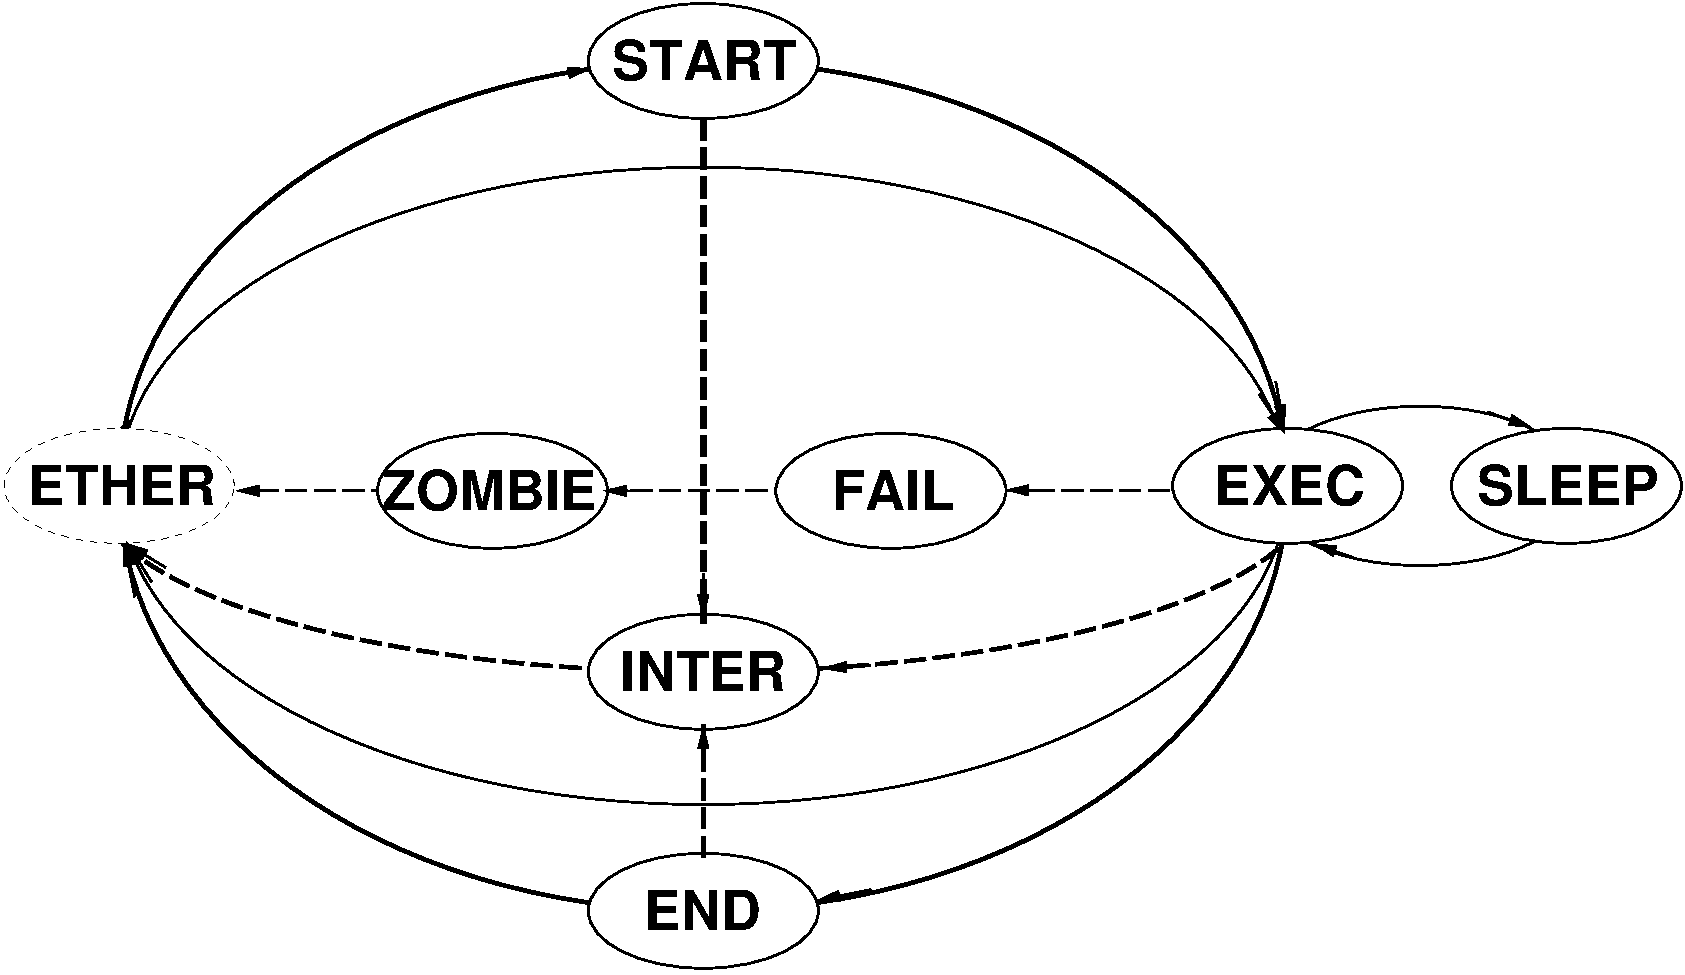
\includegraphics[width=0.8\hsize]{fig/activity-states}
\caption{States and transitions of activities.}
\label{fig|states}
\end{figure}

Note: in case of a problem, one can go into the {\tt FAIL} state, or even
directly into the {\tt ZOMBIE} state. The module is then frozen.

As of today, the  number of states is fixed  and  a future version  might
change this.  However, a workaround  is  still possible with the  current
version, by using internal   state   variables. The current  states   are
recalled in the following table:

\bigbreak

{\small\begin{tabularx}{0.8\linewidth}{|l||X|l|}
\hline
state 	& comments 	& codel (if defined)	  \\
\hline
\tt START  & startup state 
		& \tt c\_exec\_func\_start 	\\
\tt EXEC   & main execution state & \tt c\_exec\_func  \\
\tt END    & termination state 	& \tt c\_exec\_func\_end \\
\tt FAIL   & failure (and module freeze) \em 
					& \tt c\_exec\_func\_fail \\
\hline
\tt INTER  & interruption state 
					& \tt c\_exec\_func\_inter  \\
\hline
\tt SLEEP     	&  suspended activity (waits an external event to go back
into  {\tt EXEC} ) & \\
\tt ETHER    	& \em terminated activity  & \\
\tt ZOMBIE   	& \em terminated activity and frozen module & \\
\hline
\end{tabularx}}

\bigbreak

State description:

\begin{itemize}
\item {\tt START} is the first step of the execution. If the codel is not
specified, the activity goes directly into state {\tt EXEC}.
\end{itemize}

It is up  to you to define the   following transitions. To  do so, codels
must return one value of  the enum {\tt  START},  {\tt EXEC}, {\tt  END},
{\tt ETHER},  {\tt FAIL}, {\tt  ZOMBIE} or {\tt SLEEP}, which corresponds
to the state of the same name. One does normally follow the sequence {\tt
START} $\rightarrow$ {\tt   EXEC} $\rightarrow$  {\tt  END} $\rightarrow$
{\tt ETHER}.

\begin{itemize}
\item {\tt EXEC}, {\tt END} and {\tt INTER} are decribed in the previous
sections.

\item {\tt ETHER} indicates that the activity does not exist anymore.

\item {\tt ZOMBIE} indicates that the activity stopped due to an abnormal
situation. The module  is then  frozen and  will not answer  any requests
anymore. A special request {\tt Abort} let you resume the activity, which
then  goes into the  {\tt ETHER} state. This  state can  be useful if you
want  to debug  some problem.  It   can also be  useful   if you want  to
re-synchronize two modules.

\item {\tt FAIL} terminates the activity, just before going into {\tt
ZOMBIE}. The codel can do some additional cleanup.

\item {\tt SLEEP} suspends an activity, and waits for an external event
to occur (a request,  or an {\tt  h2evn} event). Then  it returns  to the
{\tt EXEC} state.
\end{itemize}

The following table summarize the possible transitions, for each state:

\bigbreak

{\small\begin{tabular}{|ll||c|c|c|c|c|c|}
\cline{3-8}
\multicolumn{2}{c}{} & \multicolumn{6}{|c|}{possible transitions} \\
\hline
state & (codel) & \tt START & \tt EXEC/SLEEP & \tt END & \tt ETHER & \tt FAIL & \tt ZOMBIE \\
\hline
\tt START  & \tt (c\_exec\_func\_start)	& X & X & X & X & X & X \\
\tt EXEC   & \tt (c\_exec\_func) 	&   & X & X & X & X & X \\
\tt END    & \tt (c\_exec\_func\_end) 	&   &   & X & X & X & X \\
\tt INTER  & \tt (c\_exec\_func\_inter) &   &   &   & X & X & X \\
\tt FAIL   & \tt (c\_exec\_func\_fail) 	&   &   &   &   & X & X \\
\hline
\end{tabular}}

Note: a termination state ({\tt END}, {\tt FAIL} or {\tt INTER}) is never
interrupted.


% =======================================================================

\section{Writing the codels}
\label{sec|codels|writing}


\subsection{Control codels  {\tt c\_control\_func}}

See        example            in           section~\ref{ssec|control|ex},
page~\pageref{ssec|control|ex}.

\subsection{Execution codels  {\tt c\_exec\_func\_*}}

Execution  codels have 1,  2 or 3  parameters,  depending on the request.
These codels can have,  in this order and   if the corresponding  data is
defined,  a pointer to  the   input structure,  a pointer  to  the output
structure and a pointer to the report (always  defined). Codels return an
{\tt ACTIVITY\_EVENT}, as exposed in the previous section.

Here is the {\tt demoGotoPosition}  execution codel ({\tt c\_exec\_func})
of the {\tt MoveDistance} request of the module {\tt demo}. This codel,
invoked periodically, controls the speed of the mobile (according to the
one specified with the {\tt SetSpeed} request), and stops when the
requested position is reached. We suppose we have two low level functions
which control the mobile:

\begin{itemize}
\item {\tt STATUS mobileState(double *position, double *speed)} which get
the current status of the mobile (thanks to sensors) and
\item {\tt STATUS mobileMove(double position, double speed)} which move
the mobile to the requested position at the requested speed.
\end{itemize}

\begin{center}\begin{cartouche}\small\begin{verbatim}
ACTIVITY_EVENT
demoGotoPosition(double *goal, int *bilan)
{
   double remain;       /* remaining distance (m) */
   double speed;        /* requested speed (m/s) */
   double increment;    /* position change (m) */

   /* Measure current speed and position */
   if (mobileState(&(SDI_F->state.position), &(SDI_F->state.speed)) != OK) {
        *bilan = S_demo_MOBILE_OUT_OF_ORDER;
        return ETHER;
   }

   /* Compute the remaining distance */
   remain = *goal - SDI_F->state.position;

   /* Get the reference speed */
   if (SDI_F->speedRef == DEMO_SLOW) 
        speed = DEMO_SLOW_SPEED;
   else
        speed = DEMO_FAST_SPEED;

   /* Compute an elementary move, according to the speed and period */
   increment = speed * DEMO_MOTION_TASK_PERIOD;

   /* Are we done? */
   if (fabs(remain) < increment) {
        if (mobileMove(*goal, 0) != OK) {
            *bilan = S_demo_MOBILE_OUT_OF_ORDER;
            return ETHER;
        }
        return END;
   }

   /* Continue */
   if (mobileMove(SDI_F->state.position +
                      SIGN(remain) * increment, speed) != OK) {
        *bilan = S_demo_MOBILE_OUT_OF_ORDER;
        return ETHER;
   }
   return EXEC;
}
\end{verbatim}\end{cartouche}\end{center}

Notes:

The {\tt SDI\_F} macro let you acces the fIDS structure.

{\tt DEMO\_MOTION\_TASK\_PERIOD} is the period of the execution task
(stored in the cIDS).

We will see later how one can access IDSs and how reports can be used.


\subsection{Initialization codel {\tt c\_init\_func}}

One initialization codel can be associated to any  execution task, by the
mean of the field {\tt  c\_init\_func}. It is  usually used to initiliaze
the fIDS to a known state. It takes only one  parameter: a pointer to the
report.   It returns either {\tt  OK}  or {\tt ERROR}  (in  that case the
module does not start).

For the {\tt demo} module,  this codel chooses  a  default speed for  the
mobile  and intializes its state.   Note  that fISD are not automatically
initialized with zeros.

The constants and default values used by a  module are usually defined in
a header file in the main directory  of the module. In  that case this is
{\tt demoConst.h}.

\begin{center}\begin{cartouche}\small\begin{verbatim}
STATUS
demoInit(int *bilan)
{
  SDI_F->state.position = 0.;
  SDI_F->state.speed = 0;
  SDI_F->distRef = 0;
  SDI_F->posRef = 0;
  SDI_F->speedRef = DEMO_SLOW;

  return OK;
}
\end{verbatim}\end{cartouche}\end{center}


\subsection{Permanent activity codel {\tt c\_func}}

A permanent activity can  be defined for  any execution task, by the mean
of the  field  {\tt c\_func}.  It is executed  each  time the task  wakes
up. It is usually used to set up a  filtering function (pose computation,
sonar echos  reading, \ldots), or   a permanent  servoing activity  which
starts and stops with the module.

This codel takes only one parameter, a pointer on the report, and returns
a {\tt STATUS} ({\tt OK} or {\tt ERROR}).  Be warned that  if an error is
returned, the execution task  is {\em suspended} (it  is resumable with a
{\tt taskResume}).

Since this activity is not associated to a  request, the report is stored
in the cIDS as well as in the control poster. Clients can read the poster
to know the status of this activity.


% =======================================================================
\section{Parallel activities and synchronization}

Execution   requests can  only  be  declared  {\em   compatible} or  {\em
incompatible} with each other. In the first case, their execution becomes
completely  independent one another.  In  the second case, they interrupt
themselves.  There are  some   intermediate  cases, where  requests  must
synchronize, or exchange  data.   Those cases are  to  be handled  by the
codels.

To  do so, it is  possible to use {\em  activity  ids}: each eactivity is
identified be a number between  $0$ and {\tt MAX\_ACTIVITIES}$-1$. From a
codel,   the current  activity number  is    returned by the  macro  {\tt
CURRENT\_ACTIVITY\_NUM}.

This  id can be  used  to exchange   information between activities.  For
instance, it would  be possible to  declare  a global (static) array,  of
size {\tt  MAX\_ACTIVITIES},    in which   each  element   would  contain
information regarding each activity  (current state, order of  arrival of
the request, number of the previous and next activity, \ldots).

Consider  the following  example,  where  you wish  to {\em  concatenate}
several motion  requests  for a   mobile.  The  motion  request  must  be
compatible with  itself (because it must not  interrupt the latest motion
request)  {\em but} the execution codel  {\tt EXEC} must not start before
the previous request has completed.  This must be handled internally, and
the  transition {\tt START}  $\rightarrow$  {\tt EXEC}  of a new activity
must be  synchronized with the  transition {\tt  EXEC} $\rightarrow$ {\tt
END} of the activity.

Such  a  synchronization     can  be  achieved   in     the   codel  {\tt
c\_exec\_func\_start}. This codel can register new activities in a global
array, attach to them the previous activity, and  stay in the {\tt START}
state  until the previous activity  stops. The latter information will be
registered by the codel {\tt c\_exec\_func\_end}.

The following  code  proposes an  example of such   start and end codels,
along with the global data definition:


\begin{center}\begin{cartouche}\small\begin{verbatim}
/* Global array for "Motion" requests */
struct DEMO_MOTION_STR {
    ACTIVITY_EVENT state;
    int next;
} demoMotionTab[MAX_ACTIVITIES] = {ETHER, -1};

/* Latest "Motion" request sent */
static int demoMotionLast = -1; 
\end{verbatim}\end{cartouche}\end{center}

\begin{center}\begin{cartouche}\small\begin{verbatim}
/* Start codel c_exec_func_start of the "Motion" activity */
ACTIVITY_EVENT
demoMotionStart(MOTION_STR *params, int *bilan)
{
    int current = CURRENT_ACTIVITY_NUM(DEMO_MOTIONTASK_NUM);

    /* If that is a new activity */
    if (demoMotionTab[current].state == ETHER) {

        /* If there is an active activity: wait */
        if (demoMotionLast != -1) {
            demoMotionTab[current].state = START;
            demoMotionTab[demoMotionLast].next = current;
        }
        /* No activity: one can start immediately */
        else {
            demoMotionTab[current].state = EXEC;
        }

        /* Append ourselves to the end of the list */
        demoMotionLast = current;
    }
    return (demoMotionTab[current].state);
}
\end{verbatim}\end{cartouche}\end{center}

\begin{center}\begin{cartouche}\small\begin{verbatim}
/* Termination codel c_exec_func_end of the "Motion" activity */
ACTIVITY_EVENT
demoMotionEnd(MOTION_STR *params, int *bilan)
{
    int current = CURRENT_ACTIVITY_NUM(DEMO_MOTIONTASK_NUM);
    int next;

    /* Next activity number */
    next = demoMotionTab[current].next;

    if (next == -1) 
       /* If there is no next activity */
        demoMotionLast = -1;
    else
       /* Unblock next activity */
        demoMotionTab[next].state = EXEC;

    /* This activity is terminated */
    demoMotionTab[current].next = -1;
    demoMotionTab[current].state = ETHER;
    return ETHER;
}
\end{verbatim}\end{cartouche}\end{center}

Warning: if   a   synchronized activity   fails (either  because   it  is
interrupted or because of a problem), it must signal  it to other pending
activities in order to also cancel them. It will also be necessary to set
up  a way to  re-synchronize  with clients,  for  instance with a control
request.


% =======================================================================
\section{Coding advice}

\subsection{General coding rules}

A  module is designed  to be  integrated in a  complex system:  users and
maintainers are usually not the same people.  For this reason, it is very
important to respect a few coding rules.

\begin{itemize}
\item Split programs into functions and files of a reasonable size;

\item Prototype functions;

\item Comment your code while you are writing it: 
   \begin{itemize}
   \item A comment for each function which documents the purpose and the
	 limitations you are aware of.
   \item A comment for an average of 3 or 4 lines of code.
   \end{itemize}

\item Avoid global variables;

\item Avoid magic numbers (use constants and {\tt \#define}).

\item Choose a uniform style, and follow it. For instance, VxWorks uses
all uppercased  words, separated by underscores  for constants (e.g. {\tt
DEMO\_SPEED}) and lowercase words, with a first uppercase letter for each
word but the first (e.g. {\tt controlSpeed}) for symbols;

\item Prefix all exported symbols (types, constants, functions, \ldots)
with e.g. the module name;

\item Use explicit names. Avoid short names such as {\tt i}, {\tt nb},
{\tt num}.

\item Check validity of input parameters and return a report in case of
an error.
\end{itemize}


\subsection{Case of embedded real-time systems}

Modules are likely  to be embedded on  a distant machine, where they will
interact  with other modules  and     processes.   This implies a     few
constraints since a  failure of your module can  affect the integrity  of
the whole system.

\begin{description}
\item[Memory limitations:]
Memory is  usually limited on  embedded systems: there is  not so often a
virtual memory system. You must thus avoid big  data structures, and {\em
free} as much as  possible unused memory. This  can be done thanks to the
{\tt END} and {\tt INTER} states of the codels.

\item[Memory sharing:]
Some  systems (e.g. VxWorks)   do not  have   private address  space  for
processes. Global data is shared among every processes  which runs on the
same CPU. You  must thus {\em  discriminate} as  much  as possible global
names.  In   such system, there   is nothing  that will   prevent  global
variables with the same name to interfere!

Furthermore, there are systems which do not provide memory access checks.
It is possible to read or write  in the whole memory,  even in the system
memory.  Array read or writes   beyond bounds will  lead to unpredictable
results...  It is very advised to  process to memory checks with adequate
tools such as {\tt workShop} or {\tt purify}.

\item[Temporal constrains:]

For activities that do have hard temporal constrains,
\begin{itemize}
\item Give a high priority to the task,
\item Avoid displays such as {\tt printf()}, which can be very time
consuming.
\item Avoid dynamic memory allocations, expensive and not necesseraly
bounded in time.  Modules generated by \GenoM\ do {\em no} dynamic memory
allocation: they execute in  constant time.  Moreover, memory  allocation
can always fail, and  thus block  an execution.  It  is  safer to do  all
allocation (static or dynamic) upon module startup.
\end{itemize} 

To  check that your  activities  do no  last   too much, you  can display
precise statistics   for  codels. See  chapter~\ref{cha|using}   in  this
document.

\item[Error recovery:]

As opposed to a  simulated  system, you  cannot   just display an   error
message and exit when you  encounter an abnormal situation.  The  message
will usually be lost (or not seen) and the whole  system can be in danger
(with potential dangerous situations for the machine).

You must thus:

\begin{enumerate}
\item Think of every possible problem (invalid parameters, case not
handled by the function, insufficient memory,  \ldots) and define reports
for every such situation.
\item Detect failures: check the parameters, check the results of
functions.
\item Always keep a sane state inside your functions: free memory, \ldots
\item Signal every problem with an appropriate error code
\item And if you display something, do not forget to precise the name of
the module and the function implied.
\end{enumerate}

\end{description}


\chapter{Using modules}
\label{cha|using}
%
% Copyright (c) 2001 LAAS/CNRS                        --  Wed Nov  7 2001
% All rights reserved.                                     Anthony Mallet
%
% This document is a translation of the French documentation of GenoM,
% originally written by Sara Fleury and Matthieu Herrb.
%
% Redistribution  and  use in source   and binary forms,  with or without
% modification, are permitted provided that  the following conditions are
% met:
%
%   1. Redistributions  of  source code must  retain  the above copyright
%      notice, this list of conditions and the following disclaimer.
%   2. Redistributions in binary form must  reproduce the above copyright
%      notice,  this list of  conditions and  the following disclaimer in
%      the  documentation   and/or  other  materials   provided with  the
%      distribution.
%
% THIS SOFTWARE IS PROVIDED BY THE  AUTHOR AND CONTRIBUTORS ``AS IS'' AND
% ANY  EXPRESS OR IMPLIED WARRANTIES, INCLUDING,  BUT NOT LIMITED TO, THE
% IMPLIED WARRANTIES   OF MERCHANTABILITY AND  FITNESS  FOR  A PARTICULAR
% PURPOSE ARE DISCLAIMED.  IN NO  EVENT SHALL THE AUTHOR OR  CONTRIBUTORS
% BE LIABLE FOR ANY DIRECT, INDIRECT,  INCIDENTAL, SPECIAL, EXEMPLARY, OR
% CONSEQUENTIAL DAMAGES (INCLUDING,  BUT  NOT LIMITED TO, PROCUREMENT  OF
% SUBSTITUTE  GOODS OR SERVICES;  LOSS   OF  USE,  DATA, OR PROFITS;   OR
% BUSINESS  INTERRUPTION) HOWEVER CAUSED AND  ON ANY THEORY OF LIABILITY,
% WHETHER IN CONTRACT, STRICT LIABILITY, OR TORT (INCLUDING NEGLIGENCE OR
% OTHERWISE) ARISING IN ANY WAY OUT OF THE  USE OF THIS SOFTWARE, EVEN IF
% ADVISED OF THE POSSIBILITY OF SUCH DAMAGE.
%
% $Id$
%

This  chapter  presents some means of  using  the services  provided by a
module and of addressing data in the posters.


% =======================================================================
\section{The interactive test program {\tt Essay}}
\label{sec|essay}

The interactive  test program  is a client  of  a module. One can  launch
several instances of it, provided they are  given different {\em numbers}
(see chapter~\ref{cha|session}).

This program proposes a menu, which associates  a number to each command:
You just have to  enter the number corresponding  to the command you want
to execute. Pressing the  {\tt  return}  key  without giving any   number
invokes the last command.

\subsection{Sending a request}

The $N$ requests of the module are numbered from $0$ to $N-1$. If a
request has some input parameters, they must be entered interactively.

The bracketed value is a default value: simply pressing {\tt return} will
select  it.  To  interrupt the interactive  input,  type  ``{\tt .}''  (a
single   dot):   defaults  values  will   be  affected   to the remaining
parameters. Default values are initialized to $0$.  Then they contain the
last entered value.

Once    you  have  entered  the   input   data, you    must  confirm  the
execution. Type ``{\tt a}'' to abort.  For an execution request, you must
choose between  the blocking mode or the  non-blocking mode. In the first
case,  the execution  of  the interactive program  will be  kept blocking
until the final reply of the request.  In the second case, the request is
just sent and  you  will be  able to  see   its final replies   later, by
yourself (with the command $77$, see below).


\subsection{Other commands}

Six other commands are defined:

\begin{description}
\item[55: posters] {\em Display posters}. This command displays another
menu, which lets view either a whole poster or a poster's sub-structure.

\item[66: abort] {\em Interrupt an activity}. This command displays the
list of running activities, and waits for the number of the activity you
wish to interrupt. Just type enter to leave this menu.

Note: if there is no running activity, you can stop the module by
entering {\tt -99}. {\tt -66} will resume suspended tasks.

\item[77: replies] {\em Read the final replies}. You must read pending
replies from time to time to empty the mailbox.

\item[88: state] {\em Display the module state}, {\em i.e.} the control
poster.

\item[99: quit] {\em Terminate the program}. But not the module!

\item[-99: end] {\em Terminate the program AND the module}.
\end{description}


% =======================================================================
\section{The interactive tcl shell {\tt tclServ}}
\label{sec|tcl}

{\tt tclServ} is  a server which  connects to  a  list of modules on  one
side, and accepts  tcl clients on  the other side.  Clients can then send
requests to  a   set   of   modules,  using the    {\tt  tcl}   scripting
language. This  can  be done  either interactively,  or  by the  mean  of
scripts.

To be able to use  this functionality, you must  generate the module with
the  option {\tt -t}.  A separate document   is (will be?) available, and
describe the usage of this server.


% =======================================================================
\section{{\tt Propice} and {\tt transGen}}
\label{sec|propice}

You must generate the module with the option {\tt -x}.
A separate document is (not yet) available.


% =======================================================================
\section{Accessing modules' posters from modules}

Two different cases must be considered.
\begin{itemize}
\item The name of the poster to be accessed is known ({\em e.g.} the
position of a mobile in the module which produces it).
\item The poster name is not known {\em a priori}, and can be dynamically
chosen.
\end{itemize}

\subsection{The poster name is known}

To be able to read such  a poster from the  codels of a module, the three
steps below must be followed:

\subsubsection{First step: ``poster\_client'' declaration}

Posters  names    must     be    declared   within    the      field {\tt
poster\_client\_from}   of each execution   task  which  will read  those
posters ({\em i.e.}  the one that runs   the codels that implement  those
functions).

For instance, the execution task named {\tt MotionTask} can be enabled to
read the poster  {\tt Mobile} from the  module {\tt demo} and  the poster
{\tt Echoes} from the module {\tt us} by stating:

\begin{center}\begin{cartouche}\small\begin{verbatim}
exec_task MotionTask {
     ...
     poster_client_from: demo::demoMobile, us::usEcho;
     ...
};
\end{verbatim}\end{cartouche}\end{center}

This declaration lets  \GenoM\ find the necessary  libraries and call the
adequate  initialization functions.


\subsubsection{Second step: reading a poster from within its clients'
codels}

From  within the  codels,   you can call  the  poster  functions   of the
libraries {\tt usPosterLib} and {\tt  demoPosterLib} (in the {\tt  auto/}
directory of  these modules).  You just  need to include  the  files {\tt
usPosterLib.h} and {\tt demoPosterLib.h} in the codels' file.

The  poster    library   provides   read   functions     (functions  {\tt
xxxPosterRead}) and display functions (functions {\tt xxxPosterShow}) for
the control and execution posters of a module.

In  the  following  example, one  first   reads   the whole poster   {\tt
demoMobile}, then only a sub-structure {\tt Ref} (see page
\pageref{typedef|demomobile} for the structure definition):

\begin{center}\begin{cartouche}\small\begin{verbatim}
   #include "demoPosterLib.h"

   DEMO_MOBILE_POSTER_STR mobile;
   double ref;

   demoMobilePosterRead(&mobile);
   demoMobileRefPosterRead(&ref);
\end{verbatim}\end{cartouche}\end{center}

These functions return a {\tt STATUS} ({\tt OK} or {\tt ERROR}). Only the
read functions have a parameter, which is the address of the structure in
which the read data will be copied.

As shown in the example, the  function name is  the concatenation of {\em
i.} the name  of  the module, {\em ii.}   the  name of the  poster  ({\tt
Cntrl} for the control poster), {\em  iii.}  the sub-structure name (when
a subpart of the poster is addressed instead of  its whole) and {\em iv.}
the suffix {\tt PosterRead} or {\tt PosterShow}.   These functions can be
found in the header {\tt demoPosterLibProto.h}.


\subsubsection{Third step: compilation}

{\bf Beware: this part might be subject to important changes}

To use libraries correspondig to other modules, you must:

\begin{itemize}
\item Define the path of this module in an {\tt Init.make} file. The
variable is the name of the module, all in uppercase letters.

For instance: {\tt DEMO = /usr/local/robots/modules/sara/demo}.

\item Add to the {\tt Makefile.unix} and {\tt Makefile.vxworks} a line
such as

 {\tt CPPFLAGS += -I\$\{DEMO\} -I\$\{DEMO\}/auto}.

\item Add to the {\tt Makefile.unix} a line like:

 {\tt LIBS += \$\{DEMO\}/auto/\$\{TARGET\}/demoClient.a}.

For VxWorks, you must load   the client library {\tt demoPosterLib.o}  or
{\tt demoClient.o} (which contains the first one).

\end{itemize}


\subsection{The poster name is not known}

If the name of the  poster to read is unknown  ({\em e.g.} if it will  be
set by a user) you  cannot use its  library. You must use basic functions
of the generic {\tt posterLib} library instead.

When, at run time,  you will get the  name of the  poster, you must first
find  its id  number,  which   is done  thanks   to the   functions  {\tt
posterFind}, as shown in the example below:

\begin{center}\begin{cartouche}\small\begin{verbatim}
   static POSTER_ID distantPosterId;
   char *name;
   ...
   if (posterFind(name, &distantPosterId) == ERROR) {
      *report = errnoGet();
   }
   ...
\end{verbatim}\end{cartouche}\end{center}

We have  already seen how to write  into posters. The read function works
in the same way:

The   {\tt  posterRead} function   has the  same    prototype as the {\tt
posterWrite} function:

\bigbreak
{\tt int posterRead(POSTER\_ID posterId, int offset, char *buf, int nbytes)}
\bigbreak

{\tt  posterId} is  the poster id   (returned by {\tt posterFind}),  {\tt
offset} is the offset  in bytes from  the beginning of the structure  and
{\tt  nBytes} is the number  of bytes to read.   The function returns the
number of bytes actually read (normally {\tt nBytes}).

As for {\tt posterWrite},  it is also possible to  use the address of the
poster and   write  directly into  it,  thanks  to  the {\tt  posterAddr}
function. Such accesses must be protected with a pair of {\tt posterTake}
and {\tt posterGive} ({\tt posterTake} must be  called with the flag {\tt
POSTER\_READ} instead of {\tt POSTER\_WRITE}).

\begin{center}\begin{cartouche}\small\begin{verbatim}
    double speed;

    posterTake(posterId, POSTER_READ);
    speed = addrPosterMotion->state.speed;
    posterGive(posterId);
\end{verbatim}\end{cartouche}\end{center}


% =======================================================================
\section{Accessing modules services from modules}

It is  possible to  send  requests to module   from any  process,  and in
particular from  other  modules ({\em i.e.} from  their  codels). As  for
posters, you must follow three steps:

\subsection{First step: declaring modules}

The modules to which you want to send requests are  to be declared in the
execution task field {\tt cs\_client\_from}. For instance, if you wish to
use the services of the modules {\tt demo} and {\tt us}:

\begin{center}\begin{cartouche}\small\begin{verbatim}
exec_task MotionTask {
     ...
     cs_client_from: demo, us;
     ...
};
\end{verbatim}\end{cartouche}\end{center}

This  step lets \GenoM\  find  the necessary communication libraries  and
automatically call  the initialization  functions (create a  mailbox, and
get a client id).

\subsection{Second step: sending requests and receiving replies}

You   can send requests from   codels  through the  functions  of the two
libraries  {\tt usMsgLib}   and {\tt  demoMsgLib}  (in  the case of   our
example). To do so, you need to include the  headers {\tt usMsgLib.h} and
{\tt demoMsgLib.h}.

The library {\tt demoMsgLib}  defines  several functions whose  names are
concatenation of: {\em i.} the name of the module, {\em  ii.} the name of
a request ({\tt  Abort} for the interrupt request),  {\em iii.} a  suffix
showing its purpose. Four suffixes are available:


\begin{center}\small\begin{tabularx}{\linewidth}{|l|X|}
\hline
suffix & function \\
\hline
\tt RqstSend & send a request (non blocking) \\

\tt ReplyRcv & receive a reply (final or intermediate)  (blocking or not)\\

\tt RqstAndRcv & send a request {\em and} receive the {\em final reply}
(blocking) \\

\tt RqstAndAck & send a request {\em and} receive the {\em intermediate reply}
(blocking) \\
\hline
\end{tabularx}\end{center}

For a  control request, you  can use  the function  {\tt RqstAndRcv} even
though it is blocking: indeed, control requests are meant to execute in a
very short time, so that the final reply should quickly occur.

However, for  an  execution request it   is strongly advised   to use the
function {\tt  RqstAndAck}, which waits only  for the  intermediate reply
(acknowledgment of the reception of the request).  In general, you cannot
block your module until the completion of the  remote request.  The final
reply will be  read with the  non-blocking function {\tt ReplyRcv}, which
you will have to call until reception of the reply.

Consider this example:

\begin{itemize}
\item To send the control request {\tt SetSpeed} to  the {\tt demo}
module, you can use the function {\tt demoSetSpeedRqstAndRcv}.

\item To send the execution request {\tt Monitor}, you can use:
   \begin{itemize}
      \item the function {\tt demoMonitorRqstAndAck} and then
      \item the function {\tt demoMonitorReplyRcv} in non-blocking mode,
until the reply comes. (if there is nothing else to do, the {\tt SLEEP}
state is particularly well suited).
   \end{itemize}
\end{itemize}

The prototypes  of  these  functions  are defined   in the  header   {\tt
auto/demoMsgLibProto.h}. Generic functions  (as for posters) also exists,
and are documented in the sections below).

\subsection{Third step: compilation}

To compile  and link under  Unix, you can use the  same procedure  as for
posters. For VxWorks, the library to load  is {\tt demoMsgLib.o}, or {\tt
demoClient.o} which includes it.


\subsection{An example}

We  present here a few  examples, which involve  a module {\tt pilo} that
must send  the {\tt  SetSpeed} and   {\tt MoveDistance}  requests  to the
module {\tt demo}. These  requests are  sent  by the execution  task {\tt
CmdTask}. The {\tt  cs\_client\_from:  demo} field has been   declared in
this task.

\subsubsection{Sending a control request: {\tt RqstAndRcv}}

The functions {\tt RqstAndRcv} can have 2, 3 or 4 arguments, depending on
the input and output declarations of the request:

\begin{center}\begin{cartouche}\small\begin{verbatim}
  int ...RqstAndRcv(CLIENT_ID clientId,
                    [STR_IN *in,] [STR_OUT *out,] int *report);
\end{verbatim}\end{cartouche}\end{center}

\begin{itemize}
\item The first argument is the client number. For instance: {\tt
PILO\_CMDTASK\_DEMO\_CLIENT\_ID} for the module {\tt pilo}, client of the
module {\tt  demo}, in the execution  task {\tt CmdTask} (see header {\tt
piloHeader.h}.

\item The second and third arguments (between square brackets) are
optional, and defined only if the request defines an input or an output
parameter.

\item The last argument is the report, returned by the request.
\end{itemize}

This function returns {\tt FINAL\_REPLY\_OK}  if everything went well, or
{\tt ERROR} if not.

\bigbreak

The following example sends the {\tt SetSpeed} request from the codel
{\tt piloSendRequest} of the module {\tt pilo}:

\begin{center}\begin{cartouche}\small\begin{verbatim}
ACTIVITY_EVENT
piloSendRequest(DEMO_SPEED *speed, int *report)
{
   if (demoSetSpeedRqstAndRcv(PILO_CMDTASK_DEMO_CLIENT_ID, 
                              speed, report) != FINAL_REPLY_OK) {
      return FAIL;
   }
   return EXEC;
}
\end{verbatim}\end{cartouche}\end{center}


\subsubsection{Sending an execution request: {\tt RqstAndAck}}

\begin{center}\begin{cartouche}\small\begin{verbatim}
  int ...RqstAndAck(CLIENT_ID clientId,
                    int *rqstId, int replyTimeOut,
                    [STR_IN *in,] [STR_OUT *out],
                    int *activity, int *report);
\end{verbatim}\end{cartouche}\end{center}

In comparison with the {\tt ...RqstAndRcv} functions, the {\tt
RqstAndAck} functions have three more arguments:

\begin{itemize}
\item {\tt rqstId} is filled with the request id. This id will let you
read the reply later.

\item {\tt replyTimeOut} is the time (in ticks) for which you want to
wait for the final reply. The value $0$ means ``wait forever''. 

\item {\tt activity} is the activity number. This number will let you get
information on it (state) or abort it.
\end{itemize}

Note: if    the execution is  very   fast, you can   get the  final reply
immediately. This is why this function also has the {\tt out} parameter.

This function returns {\tt   WAITING\_FINAL\_REPLY} if the   intermediate
reply has been received, or {\tt FINAL\_REPLY\_OK} if the final reply has
already been received. {\tt ERROR} is returned in case of a problem.

\bigbreak

The following example shows the sending of the {\tt Monitor} request from
{\tt piloSendRequest2} in the module {\tt pilo}:

\begin{center}\begin{cartouche}\small\begin{verbatim}
/* Global variables */
static int piloDemoMonitoRqstId = -1;     /* Number of the request */
static int demoMonitorActivity;           /* Number of the activity */
static double piloDemoMonitorOut;         /* Output parameter */

ACTIVITY_EVENT
piloSendRequest2(double *posMon, int *report)
{
   switch (demoMonitorRqstAndAck(PILO_CMDTASK_DEMO_CLIENT_ID, 
                                  &demoMonitorRqstId,  0,
                                  *posMon,  &piloDemoMonitorOut, 
                                  &demoMonitorActivity,  report)) {
      case WAITING_FINAL_REPLY:
         return SLEEP;
      case FINAL_REPLY_OK:
         piloDemoMonitorRqstId = -1;
         return END;
      default:
         return ZOMBIE;
  }  /* switch */
}
\end{verbatim}\end{cartouche}\end{center}


\subsubsection{Receiving replies: {\tt ReplyRcv}}

\begin{center}\begin{cartouche}\small\begin{verbatim}
  int ...ReplyRcv(CLIENT\_ID clientId,
                  int rqstId, int block,
                  [OUT *out], int *activity, int *bilan);
\end{verbatim}\end{cartouche}\end{center}

This function takes two new arguments:
\begin{itemize}
\item {\tt rqstId}, which is the identification number returned when the
request was sent,

\item {\tt block}, which tells if we want to block until the
reply arrives or not.
\end{itemize}

The  following  example shows the  reception   of the  reply of  the {\tt
Monitor}  request  from the codel   {\tt waitReply}.  We   use the static
variables defined in the previous example.


\begin{center}\begin{cartouche}\small\begin{verbatim}
ACTIVITY_EVENT
waitReply(double *posMon, int *report)
{
   switch (demoMonitorReplyRcv(PILO_CMDTASK_DEMO_CLIENT_ID, 
                             demoMonitorRqstId, NO_BLOCK,
                             &piloDemoMonitorOut, &demoMonitorActivity, 
                             &report)) {
      case WAITING_FINAL_REPLY:
         return SLEEP;
      case FINAL_REPLY_OK:
         piloDemoMonitorRqstId = -1;
         return END;
      default:
         return ZOMBIE;
  }  /* switch */
}
\end{verbatim}\end{cartouche}\end{center}

{\bf Important note:} The activity which sends  the request and reads its
reply can be interrupted.  In that case,  the codel which reads the final
reply might never be executed. It is not advised  to let such an activity
pending, without reading its reply.   To avoid this,  you must define  an
interrupt codel, in which you will  interrupt the activity started by the
initial  sending of your request.  This  can  be done  tanks  to the {\tt
Abort} request:

\begin{center}\begin{cartouche}\small\begin{verbatim}
ACTIVITY_EVENT
interActi(double *posMon, int *bilan)
{
   /* No current activity */
   if (piloDemoMonitorRqstId == -1)
         return ETHER;

   /* interrupt the Monitor activity */
   if (demoAbortRqstAndRcv(PILO_CMDTASK_DEMO_CLIENT_ID, 
                           &demoMonitorActivity, bilan) != FINAL_REPLY_OK)
         return ZOMBIE;

   /* Wait for the final reply (which should arrive shortly thanks to the
      interruption */
   if (demoMonitorReplyRcv(PILO_CMDTASK_DEMO_CLIENT_ID, 
                         demoMonitorRqstId, BLOCK_ON_FINAL_REPLY,
                         &piloDemoMonitorOut, &demoMonitorActivity, 
                         &bilan) != FINAL_REPLY_OK)
        return ZOMBIE;

   piloDemoMonitorRqstId = -1;
   return ETHER;
}
\end{verbatim}\end{cartouche}\end{center}


\section{Accessing modules services from another process}

\subsection{The library {\tt posterLib}}

The library {\tt  demoPosterLib} provides an initialization function {\tt
demoPosterInit} and a set of  read functions (ending with {\tt PosterRead})
and display  functions (ending in {\tt  PosterShow}) for the  control and
execution posters of modules.

\subsection{The library {\tt msgLib}}

Before you can use this library, you have to create a mailbox in order to
receive the replies  of remote servers. This is   done with the  function
{\tt csMboxInit}.

Then, you  must  initialize   connections  for individual    clients: for
instance {\tt demoClientInit} in the libray {\tt demoMsgLib}.

Before you  quit, you must  free this connection with {\tt demoClientEnd}
and close the mailbox with {\tt csMboxEnd}.


\chapter{GenoM syntax}
\label{cha|syntax}
%
% Copyright (c) 2001 LAAS/CNRS                        --  Wed Nov  7 2001
% All rights reserved.                                   Florent Lamiraux
%
% This document is a translation of the French documentation of GenoM,
% originally written by Sara Fleury and Matthieu Herrb.
%
% Redistribution  and  use in source   and binary forms,  with or without
% modification, are permitted provided that  the following conditions are
% met:
%
%   1. Redistributions  of  source code must  retain  the above copyright
%      notice, this list of conditions and the following disclaimer.
%   2. Redistributions in binary form must  reproduce the above copyright
%      notice,  this list of  conditions and  the following disclaimer in
%      the  documentation   and/or  other  materials   provided with  the
%      distribution.
%
% THIS SOFTWARE IS PROVIDED BY THE  AUTHOR AND CONTRIBUTORS ``AS IS'' AND
% ANY  EXPRESS OR IMPLIED WARRANTIES, INCLUDING,  BUT NOT LIMITED TO, THE
% IMPLIED WARRANTIES   OF MERCHANTABILITY AND  FITNESS  FOR  A PARTICULAR
% PURPOSE ARE DISCLAIMED.  IN NO  EVENT SHALL THE AUTHOR OR  CONTRIBUTORS
% BE LIABLE FOR ANY DIRECT, INDIRECT,  INCIDENTAL, SPECIAL, EXEMPLARY, OR
% CONSEQUENTIAL DAMAGES (INCLUDING,  BUT  NOT LIMITED TO, PROCUREMENT  OF
% SUBSTITUTE  GOODS OR SERVICES;  LOSS   OF  USE,  DATA, OR PROFITS;   OR
% BUSINESS  INTERRUPTION) HOWEVER CAUSED AND  ON ANY THEORY OF LIABILITY,
% WHETHER IN CONTRACT, STRICT LIABILITY, OR TORT (INCLUDING NEGLIGENCE OR
% OTHERWISE) ARISING IN ANY WAY OUT OF THE  USE OF THIS SOFTWARE, EVEN IF
% ADVISED OF THE POSSIBILITY OF SUCH DAMAGE.
%

This chapter gives a description of the different commands defining
a {\GenoM} module. These commands are organized into sections
corresponding to the different parts of a GenoM module.

\section{Module Declaration}
\label{sec|declaration}

\noindent
\texttt{module moduleName \{ ... \};} declaration of module with name
\texttt{moduleName}. \\

\noindent
The sub-commands of \texttt{module} are the following:

\begin{itemize}
\item[]\texttt{number:  n;} non-negative integer uniquely identifying the module in
a given control architecture.

\item[]\texttt{version:  "major.minor";} defines the version number of the
module

\item[]\texttt{email:  email;} defines the e-mail address of
the person to contact for information about this module.

\item[]\texttt{requires:  packageOrModule1 , ..., packageOrModuleN;}
specifies the dependency of the module. When generating the module,
{\GenoM} will look for \texttt{pkgconfig} input files
\texttt{packageOrModule1.pc},...,\texttt{packageOrModuleN.pc} and set
the necessary compilation flags accordingly.

\item[]\texttt{codels\_requires:  packageOrModule1 , ..., packageOrModuleN;}
specifies the dependency of the codels. When configuring the codels,
{\GenoM} will look for \texttt{pkgconfig} input files
\texttt{packageOrModule1.pc},...,\texttt{packageOrModuleN.pc} and set
the necessary compilation flags accordingly.

\item[]\texttt{lang:  "c++"} or \texttt{"c"}: specifies the programming
language with which the codels are developed.

\item[]\texttt{internal\_data}: specifies the name of the internal database.
The internal database is a standard C data-structure that should
include no pointer.

\item[]\texttt{clock\_rate}: specifies the rate of the internal clock
producing the system tick, on which period tasks are synchronized.
This declaration is optional. The default value, if not specified is
100 ticks per second.
\end{itemize}

\section{Requests}
\label{sec|requests}

\texttt{Request requestName \{ ... \};} declaration of a request with
name \texttt{requestName}.\\

\noindent
The sub-commands of \texttt{Request} are the following.\\

\begin{itemize}
\item[]\texttt{doc: }''\texttt{comment}''{\tt;} inline help of the request.
\item[]\texttt{type:  control}, \texttt{exec} or \texttt{init} defines the type of the request:
  \begin{itemize}
  \item \texttt{control}: for a control request; control requests do not
    trigger any specific action. They are mostly used for accessing the
    internal database (reading or changing parameters),
  \item \texttt{exec}: for an execution request; execution requests trigger
    (periodic or not) actions defined into execution codels,
  \item \texttt{init}: for the initialization request of the module. No
    execution request can be treated until this request has been
    called and has returned success.
  \end{itemize}

\item[]\texttt{exec\_task:  execTaskName;} defines which execution task
executes the request. Applies only for \emph{execution} and
\emph{initialization} tasks.

\item[]\texttt{input: name::idbRef;} defines the input of the
  request. \texttt{name} is the name of the variable that will be
  defined in the request codels. \texttt{idbRef} is the field of the
  internal database defining the type of the codels input. For instance:\\
\begin{verbatim}
module Test {
    internal_data:          TEST_STR;
    number:                 100;
};

typedef struct MY_STR {
  double a1;
  double a2;
} MY_STR;

typedef struct TEST_STR {
  MY_STR myStr;
} TEST_STR;

request Req {
  ...
  input:              a1::mStr.a1;
  ...
}
\end{verbatim}
defines a request with as input a \texttt{double}\\

\item[]\texttt{input\_info:  defaultValue1::"doc1" , ..., defaultValueN::"docN";}
\item[]\texttt{posters\_input:  STRUCT\_NAME\_1 , ..., STRUCT\_NAME\_N;}
specifies that the codels of the request need to read information on posters exporting
data-structures of types \texttt{STRUCT\_NAME\_1}, ...,
\texttt{  STRUCT\_NAME\_N}. {\GenoM} server part then defines functions to read
the poster with the following prototypes:\\{\small
\texttt{STATUS moduleNameSTRUCT\_NAME\_1PosterRead(POSTER\_ID posterId,
  STRUCT\_NAME\_1* x);}\\
\texttt{STATUS moduleNameSTRUCT\_NAME\_1PosterFind(char *posterName,
  POSTER\_ID *posterId);}\\
...\\
\texttt{STATUS moduleNameSTRUCT\_NAME\_NPosterRead(POSTER\_ID posterId,
  STRUCT\_NAME\_1* x);}\\
\texttt{STATUS moduleNameSTRUCT\_NAME\_NPosterFind(char *posterName,
  POSTER\_ID *posterId);}\\
}
\item[]\texttt{output:  name::idbRef;} output of the request. The type of
the output is defined by field \texttt{idbRef} of internal database
similarly as input.\\

\item[]\texttt{codel\_control: codelName;} specifies the name of the
control codel of the request. The control codel is called before
any other codels when request is triggered. If the control codel returns \texttt{ERROR}, the
request ends. The prototype of the control codels is defined by the
input and output of the request.

\item[]\texttt{codel\_start: codelName;} (only for initialization and execution
tasks.) specifies the name of the start codel of the request. Called
after the control codel. The start codel can return:
\begin{itemize}
\item \texttt{EXEC}: the function defined by \texttt{codel\_main} is called
  at the next execution period,
\item \texttt{END}: the function defined by \texttt{codel\_end} is called at the
  next execution period,
\item \texttt{ETHER}: the request terminates.
\end{itemize}

\item[]\texttt{codel\_main: codelName;} (only for initialization and execution
tasks) specifies the name of the main codel of the request. The main
codel can return:
\begin{itemize}
\item \texttt{EXEC}: the main codel is called again
  at the next execution period,
\item \texttt{END}: the function defined by \texttt{codel\_end} is called at the
  next execution period,
\item \texttt{ETHER} the request terminates.
\end{itemize}

\item[]\texttt{codel\_end:  codelName;} (only for initialization and execution
tasks) terminates request execution and returns \texttt{ETHER}.

\item[]\texttt{codel\_inter: codelName;} (only for initialization and execution
tasks) specifies the name of the interruption codel. The interruption
codel is called when the request is interrupted by another request
defined by field \texttt{interrupt\_activity}\\

\item[]\texttt{fail\_reports:  reportName1 , ..., reportNameN;}
possible error messages generated by the request. Error messages are
transformed into unique integer values stored into C macros with
names:
\begin{verbatim}
S_moduleName_reportName1, ..., S_moduleName_reportNameN
\end{verbatim}
where \texttt{moduleName} is the name of the module.

\item[]\texttt{interrupt\_activity:         RequestName1, ..., RequestNameN;}
defines the names of the requests of this module that interrupt this request when
triggered by a client. \texttt{RequestName1, ..., RequestNameN} can be
replaced by \texttt{all} to denote all the requests of the module.

\end{itemize}

\section{Posters}
\label{sec|posters}

\texttt{poster posterName \{ ... \};} declaration of poster with name
\texttt{  posterName}.\\

\noindent
The sub-commands of \texttt{poster} are the following.

\begin{itemize}
\item[]\texttt{update:  user} or \texttt{auto;} defines how the poster is updated,
either automatically (\texttt{auto}) or by the user in the codels (\texttt{user})

\item[]\texttt{type:  structName1, ..., structNameN;} defines the types of
the sub-fields of the poster. Can be used only with \texttt{update:  user;}.

\item[]\texttt{data:  name1::idbRef1 , ..., nameN::idbRefN;} defines the
types of the sub-fields of the poster by internal database fields.

\item[]\texttt{exec\_task:  taskName;} defines the name of the task that updates
the poster.

\item[]\texttt{codel\_poster\_create:  codelName;} defines the codel that creates
the poster. Can be used only with \texttt{update:  user;}.
\end{itemize}

\section{Execution Tasks}
\label{sec|exec-task}

\begin{itemize}
\item[]\texttt{exec\_task taskName \{ ... \};} defines a new execution task. The
sub-commands of an execution task declaration are the following.

\item[]\texttt{period:  number;} defines the period of the task in
ticks. The number of ticks per second is defined by the
global \texttt{clock\_rate} definition of the module.

The special value \textbf{\texttt{none}} can be used to create asynchronous
execution tasks.

\item[]\texttt{delay:  number;} defines the offset of the task with respect to
the beginning of the period.

\item[]\texttt{priority:  number;} defines the priority of the task.

\item[]\texttt{stack\_size:  size;} defines the size of the task stack.

\item[]\texttt{posters\_input:  STRUCT\_NAME\_1 , ..., STRUCT\_NAME\_N;}
specifies that the codels of the task need to read information on posters exporting
data-structures of types \texttt{STRUCT\_NAME\_1}, ...,
\texttt{STRUCT\_NAME\_N}. {\GenoM} server part then defines functions to read
the poster with the following prototypes:\\ {\small
\texttt{STATUS moduleNameSTRUCT\_NAME\_1PosterRead(POSTER\_ID posterId,
  STRUCT\_NAME\_1* x);}\\
\texttt{STATUS moduleNameSTRUCT\_NAME\_1PosterFind(char *posterName,
  POSTER\_ID *posterId);}\\
...\\
\texttt{STATUS moduleNameSTRUCT\_NAME\_NPosterRead(POSTER\_ID posterId,
  STRUCT\_NAME\_1* x);}\\
\texttt{STATUS moduleNameSTRUCT\_NAME\_NPosterFind(char *posterName,
  POSTER\_ID *posterId);}\\
}

\item[]\texttt{codel\_task\_start:  codelName;} defines the codel called at
initialization of the task when the module is launched.

\item[]\texttt{codel\_task\_end:  codelName;} defines the codel called when the task ends.

\item[]\texttt{codel\_task\_main:  codelName;} defines the codel systematically
called by the task (before all the other activities).

\item[]\texttt{codel\_task\_main2:  codelName;} defines the codel systematically
called by the task (after all the other activities).

\item[]\texttt{codel\_task\_wait: codelName}: defines a
``\emph{waiting}'' codel for asynchronous execution tasks, that is
called before \texttt{codel\_task\_main}.  When this codel
is called, it doesn't have the lock on the internal data structure of
the module. Its goal is to block the task, waiting on availability of
data on a file descriptor or a semaphore.

It's not permitted to declare a \texttt{codel\_task\_wait} codel for a
periodic task.

\item[]\texttt{fail\_reports:  reportName1 , ..., reportNameN;}
possible error messages generated by the task. Error messages are
transformed into unique integer values.
\end{itemize}


% -----------------------------------------------------------------------

\appendix

\chapter{Troubleshooting}
\label{anx|troubles}
%
% Copyright (c) 2001 LAAS/CNRS                        --  Thu Nov  8 2001
% All rights reserved.                                     Anthony Mallet
%
% This document is a translation of the French documentation of GenoM,
% originally written by Sara Fleury and Matthieu Herrb.
%
% Redistribution  and  use in source   and binary forms,  with or without
% modification, are permitted provided that  the following conditions are
% met:
%
%   1. Redistributions  of  source code must  retain  the above copyright
%      notice, this list of conditions and the following disclaimer.
%   2. Redistributions in binary form must  reproduce the above copyright
%      notice,  this list of  conditions and  the following disclaimer in
%      the  documentation   and/or  other  materials   provided with  the
%      distribution.
%
% THIS SOFTWARE IS PROVIDED BY THE  AUTHOR AND CONTRIBUTORS ``AS IS'' AND
% ANY  EXPRESS OR IMPLIED WARRANTIES, INCLUDING,  BUT NOT LIMITED TO, THE
% IMPLIED WARRANTIES   OF MERCHANTABILITY AND  FITNESS  FOR  A PARTICULAR
% PURPOSE ARE DISCLAIMED.  IN NO  EVENT SHALL THE AUTHOR OR  CONTRIBUTORS
% BE LIABLE FOR ANY DIRECT, INDIRECT,  INCIDENTAL, SPECIAL, EXEMPLARY, OR
% CONSEQUENTIAL DAMAGES (INCLUDING,  BUT  NOT LIMITED TO, PROCUREMENT  OF
% SUBSTITUTE  GOODS OR SERVICES;  LOSS   OF  USE,  DATA, OR PROFITS;   OR
% BUSINESS  INTERRUPTION) HOWEVER CAUSED AND  ON ANY THEORY OF LIABILITY,
% WHETHER IN CONTRACT, STRICT LIABILITY, OR TORT (INCLUDING NEGLIGENCE OR
% OTHERWISE) ARISING IN ANY WAY OUT OF THE  USE OF THIS SOFTWARE, EVEN IF
% ADVISED OF THE POSSIBILITY OF SUCH DAMAGE.
%
% $Id$
%

\section{Module generation}

Avoid conflicts with \GenoM\ keywords: in the \texttt{.gen} file, do not use
variables nor functions named \texttt{type}, \texttt{control}, \texttt{poster},
\ldots

Avoid conflicts with structure names which are generated by \GenoM: 
\texttt{DEMO\_STR}, \ldots

\GenoM\ should parse every valid \texttt{C} file. As of today, a few
problems remain, especially for \texttt{union}s and  recursive typedefs such as
\texttt{typedef  PILO\_MOVE\_STR PILO\_MOVE\_STR\_2[2]}.  You should not use
them at this time.

Problems may also arise if you use different names for  a structure and a
typedef associated to that structure, as in the following example:

\begin{center}\begin{cartouche}\small\begin{verbatim}
/* XXX avoid that at this time */
typedef struct DIST_STR {
   double dist;
} dist_str;
\end{verbatim}\end{cartouche}\end{center}


\section{Execution under Unix}

\subsection{\texttt{csLib} initialization failures}

\begin{center}\begin{cartouche}\small\begin{verbatim}
blues% h2 init
Initializing csLib devices: 
Cslib devices already exist on this machine.
Do you want to delete and recreate them (y/n) ? 
\end{verbatim}\end{cartouche}\end{center}

$\rightarrow$ \texttt{csLib} is already initialized.  You can answer \texttt{n}
if  everything is  ok  and  you  don't   need to initialize  \texttt{csLib}
again. Answer \texttt{y} if you need to reset \texttt{csLib}.


\subsection{Module startup failures}

\begin{center}\begin{cartouche}\small\begin{verbatim}
blues% ./codels/i386-linux/demo -b
Hilare2 execution environment version 2.11
Copyright (c) 1999-2011 LAAS/CNRS
demo: error creating /home/matthieu/.demo.pid: File exists
\end{verbatim}\end{cartouche}\end{center}

$\rightarrow$ You didn't kill properly an old instance of the module. Use
the command ``\texttt{killmodule <module-name>}''.


\begin{center}\begin{cartouche}\small\begin{verbatim}
waits[demo] ./codels/sparc-solaris/demo
DEMO :
Spawn control task ... demoCntrlTask/posterCreate:
                                              S_h2devLib_DUPLICATE_DEVICE_NAME
\end{verbatim}\end{cartouche}\end{center}

$\rightarrow$ The  control poster already  exists: an  old module was not
killed properly, see above.


\subsection{Interactive ``Test'' program failures}

The shell  blocks   after sending  a  request: launch  another  task with
another number.



\bigbreak
\textbf{Common bugs in codels}

Writes beyond  arrays'  bounds and  writes  in memory  pages  that do not
belong to you are  very common mistakes.   Use common Unix tools such  as
\texttt{valgrind} or \texttt{purify} to help debugging these issues.


\chapter{Communication libraries}
\label{anx|posters}
%
% Copyright (c) 2001 LAAS/CNRS                        --  Thu Nov  8 2001
% All rights reserved.                                     Anthony Mallet
%
% This document is a translation of the French documentation of GenoM,
% originally written by Sara Fleury and Matthieu Herrb.
%
% Redistribution  and  use in source   and binary forms,  with or without
% modification, are permitted provided that  the following conditions are
% met:
%
%   1. Redistributions  of  source code must  retain  the above copyright
%      notice, this list of conditions and the following disclaimer.
%   2. Redistributions in binary form must  reproduce the above copyright
%      notice,  this list of  conditions and  the following disclaimer in
%      the  documentation   and/or  other  materials   provided with  the
%      distribution.
%
% THIS SOFTWARE IS PROVIDED BY THE  AUTHOR AND CONTRIBUTORS ``AS IS'' AND
% ANY  EXPRESS OR IMPLIED WARRANTIES, INCLUDING,  BUT NOT LIMITED TO, THE
% IMPLIED WARRANTIES   OF MERCHANTABILITY AND  FITNESS  FOR  A PARTICULAR
% PURPOSE ARE DISCLAIMED.  IN NO  EVENT SHALL THE AUTHOR OR  CONTRIBUTORS
% BE LIABLE FOR ANY DIRECT, INDIRECT,  INCIDENTAL, SPECIAL, EXEMPLARY, OR
% CONSEQUENTIAL DAMAGES (INCLUDING,  BUT  NOT LIMITED TO, PROCUREMENT  OF
% SUBSTITUTE  GOODS OR SERVICES;  LOSS   OF  USE,  DATA, OR PROFITS;   OR
% BUSINESS  INTERRUPTION) HOWEVER CAUSED AND  ON ANY THEORY OF LIABILITY,
% WHETHER IN CONTRACT, STRICT LIABILITY, OR TORT (INCLUDING NEGLIGENCE OR
% OTHERWISE) ARISING IN ANY WAY OUT OF THE  USE OF THIS SOFTWARE, EVEN IF
% ADVISED OF THE POSSIBILITY OF SUCH DAMAGE.
%
% $Id$
%

Communication between modules is based  on two libraries: \texttt{posterLib}
for posters and \texttt{csLib} for requests.  This appendix presents a short
overview of the functions of composing these libraries.

\section{Posters and \texttt{posterLib}}

Posters are  shared memory segments, that  can be written by their owners
and read by  any process.  The  basic poster handling functions and their
prototypes are:


\begin{center}\small\begin{tabularx}{\linewidth}{|l|X|}
\hline
name		& description \\
\hline
\tt posterCreate & poster creation \\
\tt posterFind	& look for a poster id given its name\\
\tt posterWrite	& write into a poster \\
\tt posterRead  & read a poster \\
\tt posterAddr  & get the poster address \\
\tt posterTake	& take the poster semaphore  \\
\tt posterGive	& give the poster semaphore \\
\tt posterIoctl & query information about the poster (date, ...) \\
\tt posterDelete & delete a poster \\
\tt posterShow & display the state of every poster \\
\tt posterMemCreate & create a poster at the given address \\
\hline
\end{tabularx}\end{center}

\begin{center}\small\begin{tabularx}{\linewidth}{|llX|}
\hline
\tt STATUS  & \tt posterCreate & \tt (char *name,      int size, 
	                        POSTER\_ID *id); \\
\tt STATUS  & \tt posterFind   & \tt (char *name,      POSTER\_ID *id); \\
\tt int     & \tt posterWrite  & \tt (POSTER\_ID id,   int offset,
	    		        void *buf,         int size); \\
\tt int     & \tt posterRead   & \tt (POSTER\_ID id,   int offset, 
	                        void *buf,     int size); \\
\tt void *  & \tt posterAddr   & \tt (POSTER\_ID id);  \\
\tt STATUS  & \tt posterTake   & \tt (POSTER\_ID id,   POSTER\_WRITE); \\
	    & 	or    	       & \tt (POSTER\_ID id,   POSTER\_READ); \\
\tt STATUS  & \tt posterGive   & \tt (POSTER\_ID id);   \\
\tt STATUS  & \tt posterIoctl  & \tt (POSTER\_ID id, int code, char *parg); \\
\tt STATUS  & \tt posterDelete & \tt (POSTER\_ID id);  \\
\tt STATUS  & \tt posterShow   & \tt (void);  \\
\tt STATUS  & \tt posterMemCreate & \tt (char *name,  int busSpace, 
				void *pPool, int size, POSTER\_ID *id); \\
& & {\footnotesize (busSpace: POSTER\_LOCAL\_MEM,
	    POSTER\_SM\_MEM, POSTER\_VME\_A32, POSTER\_VME\_A24)} \\
\hline
\end{tabularx}\end{center}


% =======================================================================
\section{Requests and \texttt{csLib}}

Communication between modules is based  on the client/server library 
\texttt{csLib}. Messages   (requests and replies)  are   held in mailboxes  (ring
buffers).

\texttt{csLib} has the following properties:
\begin{itemize}
\item Both the sending of requests and the reception of replies can be
done in non-blocking mode.
\item The reception of a request is associated to the execution of a 
\texttt{C} function.
\item A request generates at most two replies.
\item There is no dynamic memory allocation.
\item It runs under Unix (and VxWorks).
\end{itemize}

The client side provides the following functions:

\begin{center}\small\begin{tabularx}{\linewidth}{|l|X|}
\hline
name		& description \\
\hline
\tt csClientInit 	& \\
\tt csClientRqstSend 	& Send a request\\
\tt csClientReplyRcv 	& Receive a reply\\
\hline
\end{tabularx}\end{center}


% =======================================================================
\section{Execution}

\subsubsection{Unix} Launch \texttt{h2 init}.

To  access   remote posters   (on  another  machine),  define    the 
\texttt{POSTER\_HOST} environment  variable  with the  name  of the \emph{server}
machine (there can be only one, \emph{i.e.} all the posters must be hosted
by the same machine).

The  poster server \texttt{posterServ} is  launched by \texttt{h2 init}, except
if \texttt{POSTER\_HOST} is defined.



\chapter[The files generated by GenoM]{The files generated by \GenoM}
\label{anx|files}
%
% Copyright (c) 2001 LAAS/CNRS                        --  Thu Nov  8 2001
% All rights reserved.                                     Anthony Mallet
%
% This document is a translation of the French documentation of GenoM,
% originally written by Sara Fleury and Matthieu Herrb.
%
% Redistribution  and  use in source   and binary forms,  with or without
% modification, are permitted provided that  the following conditions are
% met:
%
%   1. Redistributions  of  source code must  retain  the above copyright
%      notice, this list of conditions and the following disclaimer.
%   2. Redistributions in binary form must  reproduce the above copyright
%      notice,  this list of  conditions and  the following disclaimer in
%      the  documentation   and/or  other  materials   provided with  the
%      distribution.
%
% THIS SOFTWARE IS PROVIDED BY THE  AUTHOR AND CONTRIBUTORS ``AS IS'' AND
% ANY  EXPRESS OR IMPLIED WARRANTIES, INCLUDING,  BUT NOT LIMITED TO, THE
% IMPLIED WARRANTIES   OF MERCHANTABILITY AND  FITNESS  FOR  A PARTICULAR
% PURPOSE ARE DISCLAIMED.  IN NO  EVENT SHALL THE AUTHOR OR  CONTRIBUTORS
% BE LIABLE FOR ANY DIRECT, INDIRECT,  INCIDENTAL, SPECIAL, EXEMPLARY, OR
% CONSEQUENTIAL DAMAGES (INCLUDING,  BUT  NOT LIMITED TO, PROCUREMENT  OF
% SUBSTITUTE  GOODS OR SERVICES;  LOSS   OF  USE,  DATA, OR PROFITS;   OR
% BUSINESS  INTERRUPTION) HOWEVER CAUSED AND  ON ANY THEORY OF LIABILITY,
% WHETHER IN CONTRACT, STRICT LIABILITY, OR TORT (INCLUDING NEGLIGENCE OR
% OTHERWISE) ARISING IN ANY WAY OUT OF THE  USE OF THIS SOFTWARE, EVEN IF
% ADVISED OF THE POSSIBILITY OF SUCH DAMAGE.
%
% $Id$
%

This appendix presents  a description of  the files  generated by \GenoM\
(source files and compiled libraries).

\textbf{XXX still not fully up-to-date}

\section{Source files in \texttt{server/}}

\begin{center}\small
 \begin{tabularx}{\linewidth}{|l|X|}
 \hline
 \multicolumn{2}{|l|}{Server side: } \\
 \hline
 \texttt{demoCntrlTask.c}& control task \\
 \texttt{demoMotionTask.c}& execution task \texttt{MotionTask}  \\
 \texttt{demoHeader.h}&  constants and macros for IDSs (\emph{must included
in the codels}). \\
 \texttt{demoType.h}&  C structures of the module
 (included by \texttt{demoHeader.h}). \\ 
 \texttt{demoModuleInit.c}& module startup. \\
 \texttt{demoInit.c}& initialization request.  \\
 \hline
 \multicolumn{2}{l}{} \\

 \hline
 \multicolumn{2}{|l|}{Client side: } \\
 \hline
 \texttt{demoMsgLib.[ch]}  &  Requests libraries. \\
 \texttt{demoConnectLib.c}  &  Smaller version of the library 
\texttt{demoMsgLib.c}: use this if you use \texttt{csLib} directly. \\
 \texttt{demoPosterLib.[ch]}  &  Posters libraries.\\
 \texttt{demoError.h}  &  Error codes (reports).\\
 \hline
 \multicolumn{2}{l}{} \\

 \hline
 \multicolumn{2}{|l|}{Test program:} \\
 \hline
 \texttt{demoTest.c}  &  interactive test program\\
 \texttt{demoScan.[ch]}  &  interactive  scan of input structures\\
 \texttt{demoPrint.[ch]}  &  display the C structures of the module\\
 \hline
 \multicolumn{2}{l}{} \\

 \hline
 \multicolumn{2}{|l|}{Tcl :} \\
 \hline
 \texttt{demoClient.tcl}  &  tcl scripts for request definition\\
 \texttt{demoTcl.c}  &   \texttt{tclServ} server functions\\
 \hline
 \multicolumn{2}{l}{} \\

 \hline
 \multicolumn{2}{|l|}{OpenPRS:} \\
 \hline
 \texttt{openprs/}  & \\
 \hline
 \multicolumn{2}{l}{} \\

 \hline
 \multicolumn{2}{|l|}{Tclserv Client:} \\
 \hline
 \texttt{tclservClient/demoTclservClientDecode.c}  & Transform string returned by \texttt{tclserv} into a C structure\\
 \texttt{tclservClient/demoTclservClientEncode.c}  & Transform a C structure into a string for \texttt{tclserv} \\
 \texttt{tclservClient/demoTclservClientMsgLib.c} & Use it to control modules using \texttt{tclserv} protocol\\
 \texttt{tclservClient/demoError.c} & Encode and decode module error encoded
 by \texttt{tclserv} protocol \\
 \hline
 \multicolumn{2}{l}{} \\
 \end{tabularx}
\end{center}

% =======================================================================
\vfill\eject
\section{Binary files}

\begin{itemize}

\item Libraries:

	\begin{itemize}
	\item Server side:

		\vspace{.3cm}
		{\small
		\begin{tabular}{ll}
		\cline{1-1}
		\tt demoCntrlTask.o &
			\multirow{3}{3.5cm}{\
			$\left.{\vrule width 0pt height .6cm} \right\}$ \
			\tt demoServeur.a} \\
		\tt demoDeplacementTask.o \\
		\tt demoModuleInit.o	\\
		\cline{1-1}
		\tt demoInit.o		
		    & 	\multirow{1}{3.5cm}{\
		      	$\left.{\vrule width 0pt} \right\}$
		      	\tt ~demoInit*}  \\
		\cline{1-1}
		\end{tabular}
		}
		\vspace{.3cm}

	\item Client side:

		\vspace{.3cm}
		{\small
		\begin{tabular}{ll}
		\cline{1-1}
		\tt demoConnectLib.o \\
		\cline{1-1}
		\tt demoTest.o 
		    & 	\multirow{1}{3.5cm}{
		      	$\left.{\vrule width 0pt} \right\}$
		      	\tt ~demoTest*}  \\
		\cline{1-1}
		\tt demoScan.o	
		    &	\multirow{4}{3.5cm}{
			$\left.{\vrule width 0pt height .8cm} \right\}$
			\tt demoClient.a}\\
		\tt demoPrint.o		\\
		\tt demoMsgLib.o	\\
		\tt demoPosterLib.o	\\
		\cline{1-1}
		\end{tabular}
		}
	\end{itemize}

\end{itemize}


% -----------------------------------------------------------------------


\end{document}
